\documentclass[man]{apa6}

\usepackage{amssymb,amsmath}
\usepackage{ifxetex,ifluatex}
\usepackage{fixltx2e} % provides \textsubscript
\ifnum 0\ifxetex 1\fi\ifluatex 1\fi=0 % if pdftex
  \usepackage[T1]{fontenc}
  \usepackage[utf8]{inputenc}
\else % if luatex or xelatex
  \ifxetex
    \usepackage{mathspec}
    \usepackage{xltxtra,xunicode}
  \else
    \usepackage{fontspec}
  \fi
  \defaultfontfeatures{Mapping=tex-text,Scale=MatchLowercase}
  \newcommand{\euro}{€}
\fi
% use upquote if available, for straight quotes in verbatim environments
\IfFileExists{upquote.sty}{\usepackage{upquote}}{}
% use microtype if available
\IfFileExists{microtype.sty}{\usepackage{microtype}}{}
\usepackage{color}
\usepackage{fancyvrb}
\newcommand{\VerbBar}{|}
\newcommand{\VERB}{\Verb[commandchars=\\\{\}]}
\DefineVerbatimEnvironment{Highlighting}{Verbatim}{commandchars=\\\{\}}
% Add ',fontsize=\small' for more characters per line
\usepackage{framed}
\definecolor{shadecolor}{RGB}{248,248,248}
\newenvironment{Shaded}{\begin{snugshade}}{\end{snugshade}}
\newcommand{\KeywordTok}[1]{\textcolor[rgb]{0.13,0.29,0.53}{\textbf{#1}}}
\newcommand{\DataTypeTok}[1]{\textcolor[rgb]{0.13,0.29,0.53}{#1}}
\newcommand{\DecValTok}[1]{\textcolor[rgb]{0.00,0.00,0.81}{#1}}
\newcommand{\BaseNTok}[1]{\textcolor[rgb]{0.00,0.00,0.81}{#1}}
\newcommand{\FloatTok}[1]{\textcolor[rgb]{0.00,0.00,0.81}{#1}}
\newcommand{\ConstantTok}[1]{\textcolor[rgb]{0.00,0.00,0.00}{#1}}
\newcommand{\CharTok}[1]{\textcolor[rgb]{0.31,0.60,0.02}{#1}}
\newcommand{\SpecialCharTok}[1]{\textcolor[rgb]{0.00,0.00,0.00}{#1}}
\newcommand{\StringTok}[1]{\textcolor[rgb]{0.31,0.60,0.02}{#1}}
\newcommand{\VerbatimStringTok}[1]{\textcolor[rgb]{0.31,0.60,0.02}{#1}}
\newcommand{\SpecialStringTok}[1]{\textcolor[rgb]{0.31,0.60,0.02}{#1}}
\newcommand{\ImportTok}[1]{#1}
\newcommand{\CommentTok}[1]{\textcolor[rgb]{0.56,0.35,0.01}{\textit{#1}}}
\newcommand{\DocumentationTok}[1]{\textcolor[rgb]{0.56,0.35,0.01}{\textbf{\textit{#1}}}}
\newcommand{\AnnotationTok}[1]{\textcolor[rgb]{0.56,0.35,0.01}{\textbf{\textit{#1}}}}
\newcommand{\CommentVarTok}[1]{\textcolor[rgb]{0.56,0.35,0.01}{\textbf{\textit{#1}}}}
\newcommand{\OtherTok}[1]{\textcolor[rgb]{0.56,0.35,0.01}{#1}}
\newcommand{\FunctionTok}[1]{\textcolor[rgb]{0.00,0.00,0.00}{#1}}
\newcommand{\VariableTok}[1]{\textcolor[rgb]{0.00,0.00,0.00}{#1}}
\newcommand{\ControlFlowTok}[1]{\textcolor[rgb]{0.13,0.29,0.53}{\textbf{#1}}}
\newcommand{\OperatorTok}[1]{\textcolor[rgb]{0.81,0.36,0.00}{\textbf{#1}}}
\newcommand{\BuiltInTok}[1]{#1}
\newcommand{\ExtensionTok}[1]{#1}
\newcommand{\PreprocessorTok}[1]{\textcolor[rgb]{0.56,0.35,0.01}{\textit{#1}}}
\newcommand{\AttributeTok}[1]{\textcolor[rgb]{0.77,0.63,0.00}{#1}}
\newcommand{\RegionMarkerTok}[1]{#1}
\newcommand{\InformationTok}[1]{\textcolor[rgb]{0.56,0.35,0.01}{\textbf{\textit{#1}}}}
\newcommand{\WarningTok}[1]{\textcolor[rgb]{0.56,0.35,0.01}{\textbf{\textit{#1}}}}
\newcommand{\AlertTok}[1]{\textcolor[rgb]{0.94,0.16,0.16}{#1}}
\newcommand{\ErrorTok}[1]{\textcolor[rgb]{0.64,0.00,0.00}{\textbf{#1}}}
\newcommand{\NormalTok}[1]{#1}

% Table formatting
\usepackage{longtable, booktabs}
\usepackage{lscape}
% \usepackage[counterclockwise]{rotating}   % Landscape page setup for large tables
\usepackage{multirow}		% Table styling
\usepackage{tabularx}		% Control Column width
\usepackage[flushleft]{threeparttable}	% Allows for three part tables with a specified notes section
\usepackage{threeparttablex}            % Lets threeparttable work with longtable

% Create new environments so endfloat can handle them
% \newenvironment{ltable}
%   {\begin{landscape}\begin{center}\begin{threeparttable}}
%   {\end{threeparttable}\end{center}\end{landscape}}

\newenvironment{lltable}
  {\begin{landscape}\begin{center}\begin{ThreePartTable}}
  {\end{ThreePartTable}\end{center}\end{landscape}}

  \usepackage{ifthen} % Only add declarations when endfloat package is loaded
  \ifthenelse{\equal{\string man}{\string man}}{%
   \DeclareDelayedFloatFlavor{ThreePartTable}{table} % Make endfloat play with longtable
   % \DeclareDelayedFloatFlavor{ltable}{table} % Make endfloat play with lscape
   \DeclareDelayedFloatFlavor{lltable}{table} % Make endfloat play with lscape & longtable
  }{}%



% The following enables adjusting longtable caption width to table width
% Solution found at http://golatex.de/longtable-mit-caption-so-breit-wie-die-tabelle-t15767.html
\makeatletter
\newcommand\LastLTentrywidth{1em}
\newlength\longtablewidth
\setlength{\longtablewidth}{1in}
\newcommand\getlongtablewidth{%
 \begingroup
  \ifcsname LT@\roman{LT@tables}\endcsname
  \global\longtablewidth=0pt
  \renewcommand\LT@entry[2]{\global\advance\longtablewidth by ##2\relax\gdef\LastLTentrywidth{##2}}%
  \@nameuse{LT@\roman{LT@tables}}%
  \fi
\endgroup}


\ifxetex
  \usepackage[setpagesize=false, % page size defined by xetex
              unicode=false, % unicode breaks when used with xetex
              xetex]{hyperref}
\else
  \usepackage[unicode=true]{hyperref}
\fi
\hypersetup{breaklinks=true,
            pdfauthor={},
            pdftitle={Handling missing data in smartphone location logs},
            colorlinks=true,
            citecolor=blue,
            urlcolor=blue,
            linkcolor=black,
            pdfborder={0 0 0}}
\urlstyle{same}  % don't use monospace font for urls

\setlength{\parindent}{0pt}
%\setlength{\parskip}{0pt plus 0pt minus 0pt}

\setlength{\emergencystretch}{3em}  % prevent overfull lines


% Manuscript styling
\captionsetup{font=singlespacing,justification=justified}
\usepackage{csquotes}
\usepackage{upgreek}

 % Line numbering
  \usepackage{lineno}
  \linenumbers


\usepackage{tikz} % Variable definition to generate author note

% fix for \tightlist problem in pandoc 1.14
\providecommand{\tightlist}{%
  \setlength{\itemsep}{0pt}\setlength{\parskip}{0pt}}

% Essential manuscript parts
  \title{Handling missing data in smartphone location logs}

  \shorttitle{Missing Data in Smartphone Location Logs}


  \author{Boaz Sobrado\textsuperscript{1}}

  % \def\affdep{{""}}%
  % \def\affcity{{""}}%

  \affiliation{
    \vspace{0.5cm}
          \textsuperscript{1} Utrecht University  }

  \authornote{
    Department of Methodology \& Statistics
    
    Submitted as a research report conforming to APA manuscript guidelines
    (6th edition).
    
    Correspondence concerning this article should be addressed to Boaz
    Sobrado, . E-mail:
    \href{mailto:boaz@boazsobrado.com}{\nolinkurl{boaz@boazsobrado.com}}
  }


  \abstract{Personal mobility, or how people move in their environment, is
associated with a vast range of behavioural traits and outcomes, such as
socioeconomic status, personality and mental health. The widespread
adoption of location-sensor equipped smartphones has generated a wealth
of objective personal mobility data. Nonetheless, smartphone collected
personal mobility data has remained underutilised in behavioural
research, partly due to the practical difficulties associated with
obtaining the data and partly because of the methodological complexity
associated with analysing it. Recent changes in European regulation have
made it easier for researchers to obtain this data, but the
methodological difficulties remain. The difficulty lies in that
smartphone location data is irregularly sampled, sparse and often
inaccurate. This results in a high proportion of missing data and
significant noise. In this paper we present a method called Personal Map
Matched Imputation (PPMI) to deal with missing data and noise in
smartphone location logs. The main innovation of PPMI is that it creates
a personalised spatial map for each individual based on all the
available data. In doing so PPMI leverages the regularity of human
mobility in order to smoothen noisy measurments and impute missing data
values. By simulating missing periods in real data we find that a simple
implementation of PPMI performs as well as existing methods for short (5
minute) missing intervals and substantially better for longer (1 day)
missing intervals. When imputing a subset of real missing data where
travel logs are available as a reference points, we find that PPMI
performs substantially better than existing models.}
  \keywords{Missing Data, Measurement Bias, GPS, Human Mobility \\

    \indent Word count: 2297
  }





\usepackage{amsthm}
\newtheorem{theorem}{Theorem}[section]
\newtheorem{lemma}{Lemma}[section]
\theoremstyle{definition}
\newtheorem{definition}{Definition}[section]
\newtheorem{corollary}{Corollary}[section]
\newtheorem{proposition}{Proposition}[section]
\theoremstyle{definition}
\newtheorem{example}{Example}[section]
\theoremstyle{definition}
\newtheorem{exercise}{Exercise}[section]
\theoremstyle{remark}
\newtheorem*{remark}{Remark}
\newtheorem*{solution}{Solution}
\begin{document}

\maketitle

\setcounter{secnumdepth}{0}



\section{Introduction}\label{introduction}

Why is human mobility important? How people move about in their
environment affects a wide range of outcomes, such as health, income and
social capital (Goodchild \& Janelle, 2010). Therefore it is
unsurprising that social scientists in numerous fields and even
policymakers are interested in human mobility measures. The most widely
administered personality questionnaires ask individuals to what extent
they agree with statements such as \enquote{I love large parties},
\enquote{I prefer going to the movies to watching videos at home} and
\enquote{I love to travel to places that I have never been before}
({\textbf{???}}). In economic research, the postal code of an
individual's home address is often used as a proxy for socioeconomic
status (e.g. Villanueva \& Aggarwal, 2013). Moreover, economists study
geographic labour mobility extensively (e.g. {\textbf{???}}). In fact,
the European Commission considers labour mobility important enough to
warrant its own directorate ({\textbf{???}}). The extensive use of
measures like these across different domains strongly suggests that
mobility metrics are linked to real world outcomes. Perhaps it is
unsurprising that behavioural researchers have found that mobility
measures can be used to predict academic performance (Wang, Harari, Hao,
Zhou, \& Campbell, 2015), the incidence of obesity (Zenk, Schulz, \&
Odoms-Young, 2009) or even the onset of a depressive episode in bipolar
depression patients (Palmius et al., 2017). Indeed, there is an argument
to be made that perhaps psychologists have not been studying mobility
enough. When studying behavioural differences within individuals
behavioural scientists have often neglected the fact that individuals
vary not only over time but also over space. To fully understand
behaviour we must understand how behaviour can vary across environments.

Despite the importance of mobility measures, the majority of these
measures are obtained through the use of questionnaires (such as the
IPIP) or specifically through pen-and-paper travel diaries.
Questionnaires and travel diaries are have well-known methodological
flaws: they are burdensome to collect and rely on accurate
self-reporting. The burdensomeness stems from the fact that participants
must be explicitly asked to report on their movement patterns at
frequent intervals due to forgetfulness. This makes the data expensive
to collect and limits the extent of data collection in practice. In
addition, the frequent reporting duties of the participant may bias the
participants behaviour. Participant forgetfulness also limits the
accuracy of self reported measures. There is clear evidence that
participants are systematically biased when self-reporting mobility
measures. For instance, participants under-report the frequency of short
trips (Wolf, Oliveira, \& Thompson, 2003) and underestimate the duration
of regular commutes (Delclòs-Alió, Marquet, \& Miralles-Guasch, 2017).
These obstacles can be overcome by using objective data on human
mobility.

Social scientists now have the unprecedented opportunity to easily
obtain objective data on human mobility from smartphones. Before
smartphones the only way to collect objective data on human mobility
involved giving participants an expensive professional-grade location
sensor and convincing them to take it with themselves at all times.
Barnett and Onnela (2016) points out that introducing a new device to
the participant's life may bias their behaviour. Moreover, collecting
data in such a way is costly, places a high burden on participants and
therefore the logs do not span a long time {[}Barnett and Onnela (2016).
Today millions of individuals carry smartphones with themselves every
day and do not need to be encouraged to do so by researchers.
Smartphones are equipped with a range of sensors that can be used to
track the location of the device at all times. These smartphones can
collect and store hundreds of location measurements a day. For instance,
Google Location History contains movement information on millions of
users, often spanning years (Location History, 2017). Moreover, recent
changes in EU regulations with regard to consumer data-portability
rights ensure that a willing participant should be able to easily share
this information with researchers at no cost to the either the
participant or the researchers (Commission, 2017). Taken together, this
means that researchers now have at their disposal the ability to easily
access the objective human mobility data of millions of individuals
spanning several years at little cost and without a significant burden
of the participants.

This paper wishes to achieve four objectives: First, we have argued that
understanding human mobility is important. Secondly, we argued that
social scientists should leverage data logs from smartphones to study
human mobility, instead of relying on out-dated pen-and-paper
questionnaires. Now we will explore the practical difficulties in using
smartphone location logs. Finally we will introduce Personal Map Matched
Imputation (PPMI), a method for surmounting these difficulties. We will
compare PPMI to existing methods in the literature.

\section{Background}\label{background}

Smartphone location measures are obtained primarily (but not
exclusively) by Global Positioning System (GPS) measurements. A GPS
sensor uses the distance between a device and several satellites to
determine the location of the device. Although using a GPS sensor is the
most accurate way to establish location on a smartphone, the GPS sensor
is also the most energy consuming sensor on most smartphones (M. Y. Chen
et al., 2006; LaMarca et al., 2005). In order to avoid battery depletion
and to overcome computational constraints smartphones also use
less-accurate heuristics such as WiFi access points and cellphone tower
triangulation. Smartphone location logs contain measurements from all of
these sources, usually in the form of time-stamped latitude, longitude
and accuracy values. The accuracy \(a\) of any given measurement is
given in meters such that it represents the radius of a 67\% confidence
circle (Location History, 2017). In other words, the true location of a
device should be within the radius \(a\) of the measurement 67\% of the
time.

Researchers often develop custom-made tracking applications which
participants are instructed to download on their phone. Alternatively
participants are given a phone to use for a given period of time with
the custom-made tracking app pre-installed. We call location logs
resulting from these custom-made apps \emph{custom logs}. The advantage
of custom logs is that the researchers can adjust tracking parameters,
such as the the frequency of measurements and the sensor with which they
are made. The disadvantage with this approach is that researchers have
to develop or adapt a custom-made tracking application (which is not
easy given hundreds of different types of smartphone models), distribute
it among research participants and enforce participation. Participants
may dislike tracking apps because they view them as more intrusive and
these apps regularly drain the battery of the device (G. M. Harari et
al., 2016). Moreover, researchers have distribute this application among
research participants and convince them not to turn it off.

We focus on another solution, which is to take advantage of existing
smartphone location logs (\emph{secondary logs}) . The advantages are
clear: repositories such as Google's Location History contains
information on millions of users spanning years (Location History,
2017), participants can share the data by the click of a button and
there can be no behavioural changes due to participation in the study as
the participant share past data. The disadvantage is that researchers
have no control over the tracking parameters, often resulting in logs
with sparse and inaccurate measurements. Hence, two important challenges
are dealing with missing data and measurement noise.

In order to work with secondary logs, researchers need to be able to
handle the data sparsity that leads to missing data. Missing data is a
pervasive issue in secondary logs as it can arise due to several
reasons. Technical reasons include signal loss, battery failure and
device failure. Behavioural reasons include leaving the phone at home or
switching the device off. As a result, secondary logs often contain wide
temporal gaps with no measurements. For instance, several research
groups studying mental health report missing data rates between 30\% to
50\% (Grünerbl et al., 2015; Palmius et al., 2017; Saeb et al., 2015).
Other researchers report similar trends in different fields (e.g. G. M.
Harari et al., 2016; Jankowska, Schipperijn, \& Kerr, 2015). In Figure
\ref{fig:longMeasurementsPerDay} shows that despite the long duration of
the log the sparsity it is also evident.

\begin{figure}
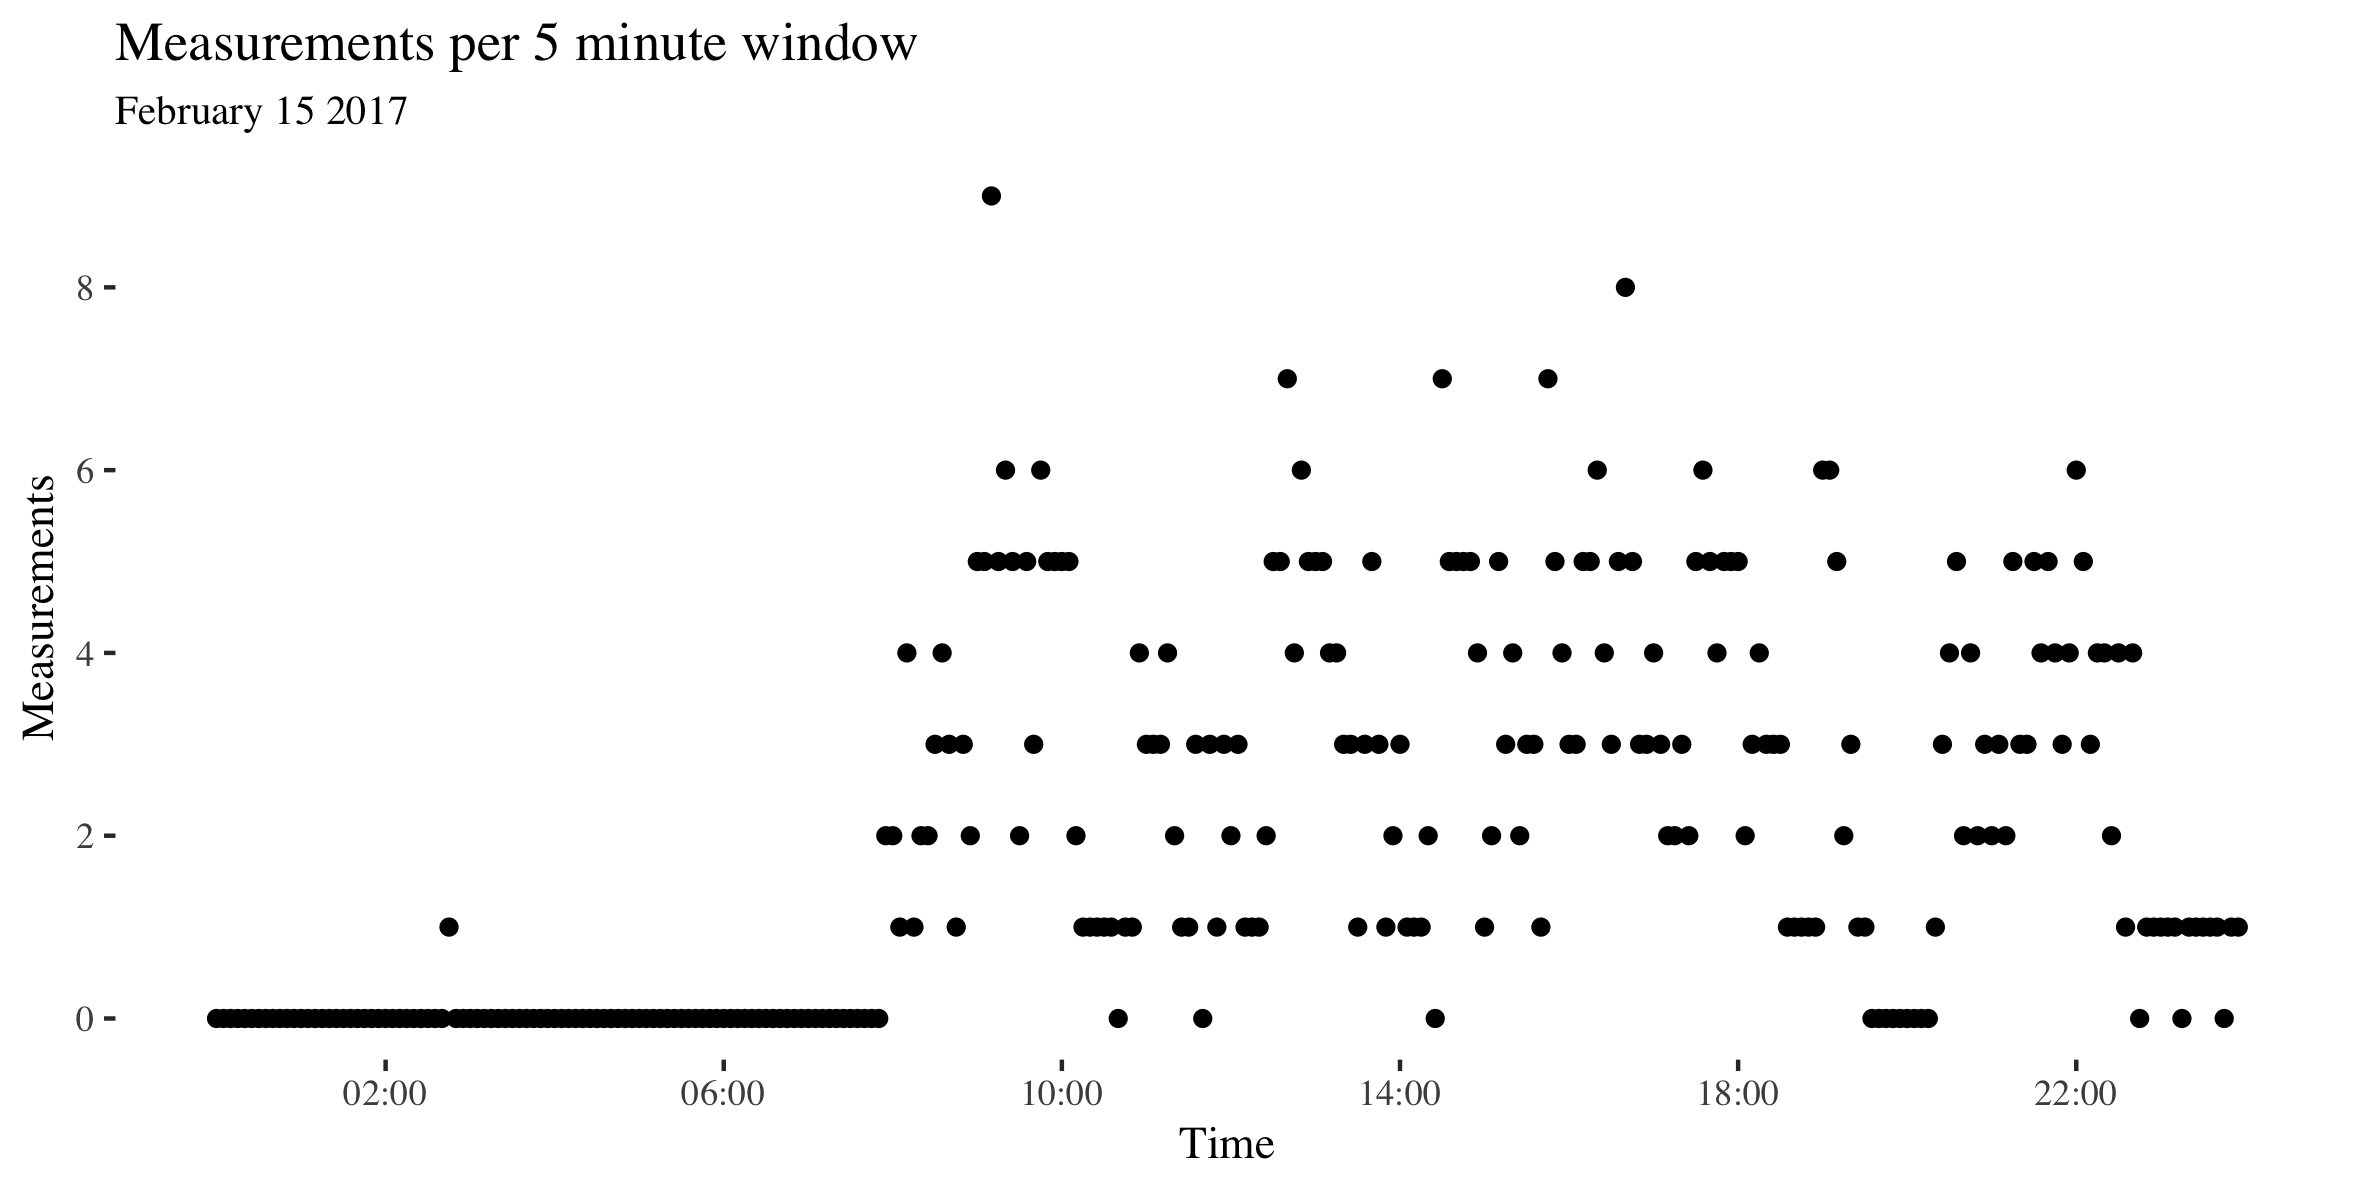
\includegraphics[width=1\linewidth]{img/missin5minExample2018} \caption{Example of missing data over the entire duration of a secondary log. The x-axis denotes time, the y-axis shows how many measurements are made and each point is a five minute window. For this day there were several periods with no information. These points lie on the x-axis.}\label{fig:longMeasurementsPerDay}
\end{figure}

There is no golden standard for dealing with missing data in GPS logs
(Barnett \& Onnela, 2016). Importantly, spatiotemporal data measurements
are auto-correlated in both time and space. This means that best
practices with other types of data, such as mean imputation, are
unsuitable. For example, imagine an individual who splits almost all her
time between work and home. Suppose she spends a small amount of time
commuting between the two along a circular path. Using mean imputation
to estimate her missing coordinates, we impute her to be at the midpoint
between home and work, even though she has never been there. Worryingly,
there is little transparency on how researchers deal with missing data
(Jankowska et al., 2015).

Another methodological problem is related to the noise in the
measurements that are collected. The accuracy of smartphone location
measurements is substantially lower than that of professional GPS
location trackers because smartphones often use less accurate sensors.
In professional GPS trackers less than 80\% of measurements fall within
10 meters of the true location. GPS measures are most inaccurate in
dense urban locations and indoors (S. Duncan et al., 2013; Schipperijn
et al., 2014). Unfortunately for researchers, this is where people in
the developed world spend most of their time. Figure
\ref{fig:accuracyPlot} shows how accuracy can vary as a function of user
behaviour, time and location. Most notably, low accuracy is often (but
not always) associated with movement (see Figure
\ref{fig:accuracyPlot2}).

\begin{figure}
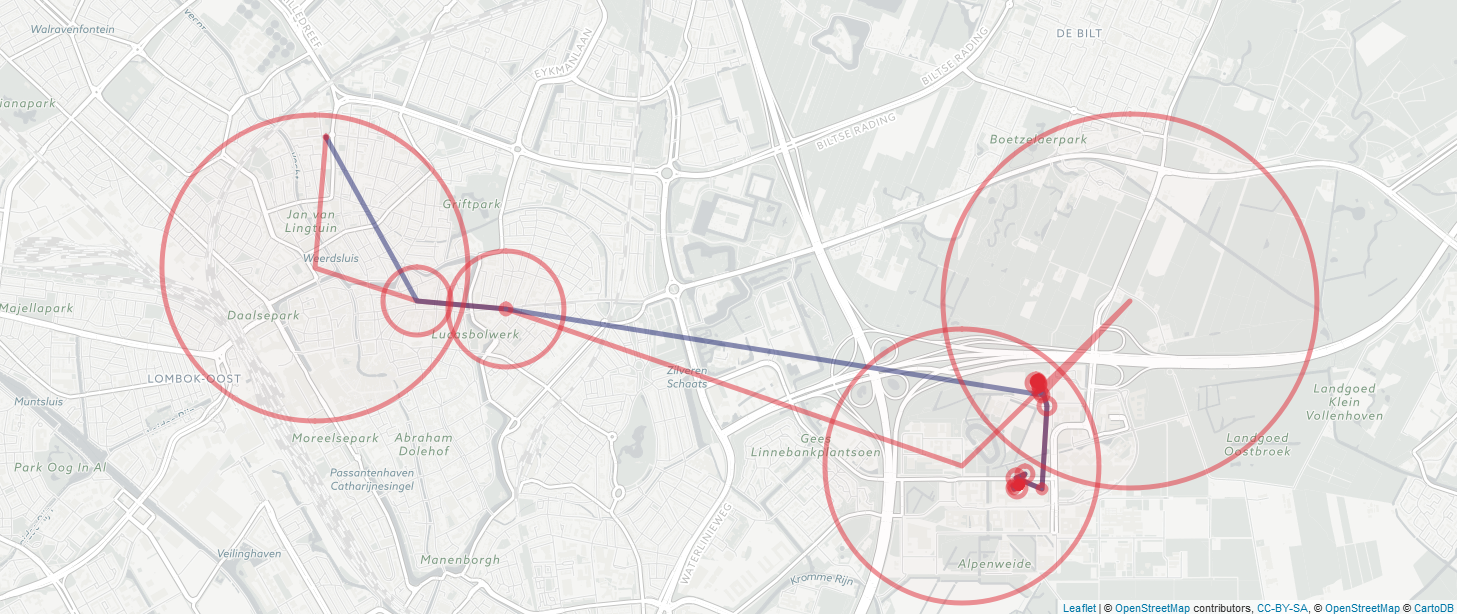
\includegraphics[width=1\linewidth]{img/journeyTillMiddayBoaz} \caption{Measurement accuracy of each logged measurement of a morning journey on February 15th 2017. This includes all measurements from midnight to midday. The red circles denote the accuracy of all logged measurement points (the raw data). The points connected in time are connected by a line. The blue line shows the path without the most inaccurate (accuracy > 400 meters) points filtered out. The red line shows the path with all measurements included. In smartphone logs inaccurate location values are interspersed between more accurate location values at higher sample rates per hour. Inaccurate measures are often followed by more accurate measures. There are several recurring low-accuracy points, such as the one in the northwest corner, possibly the result of cellphone tower triangulation.}\label{fig:accuracyPlot}
\end{figure}

\begin{figure}
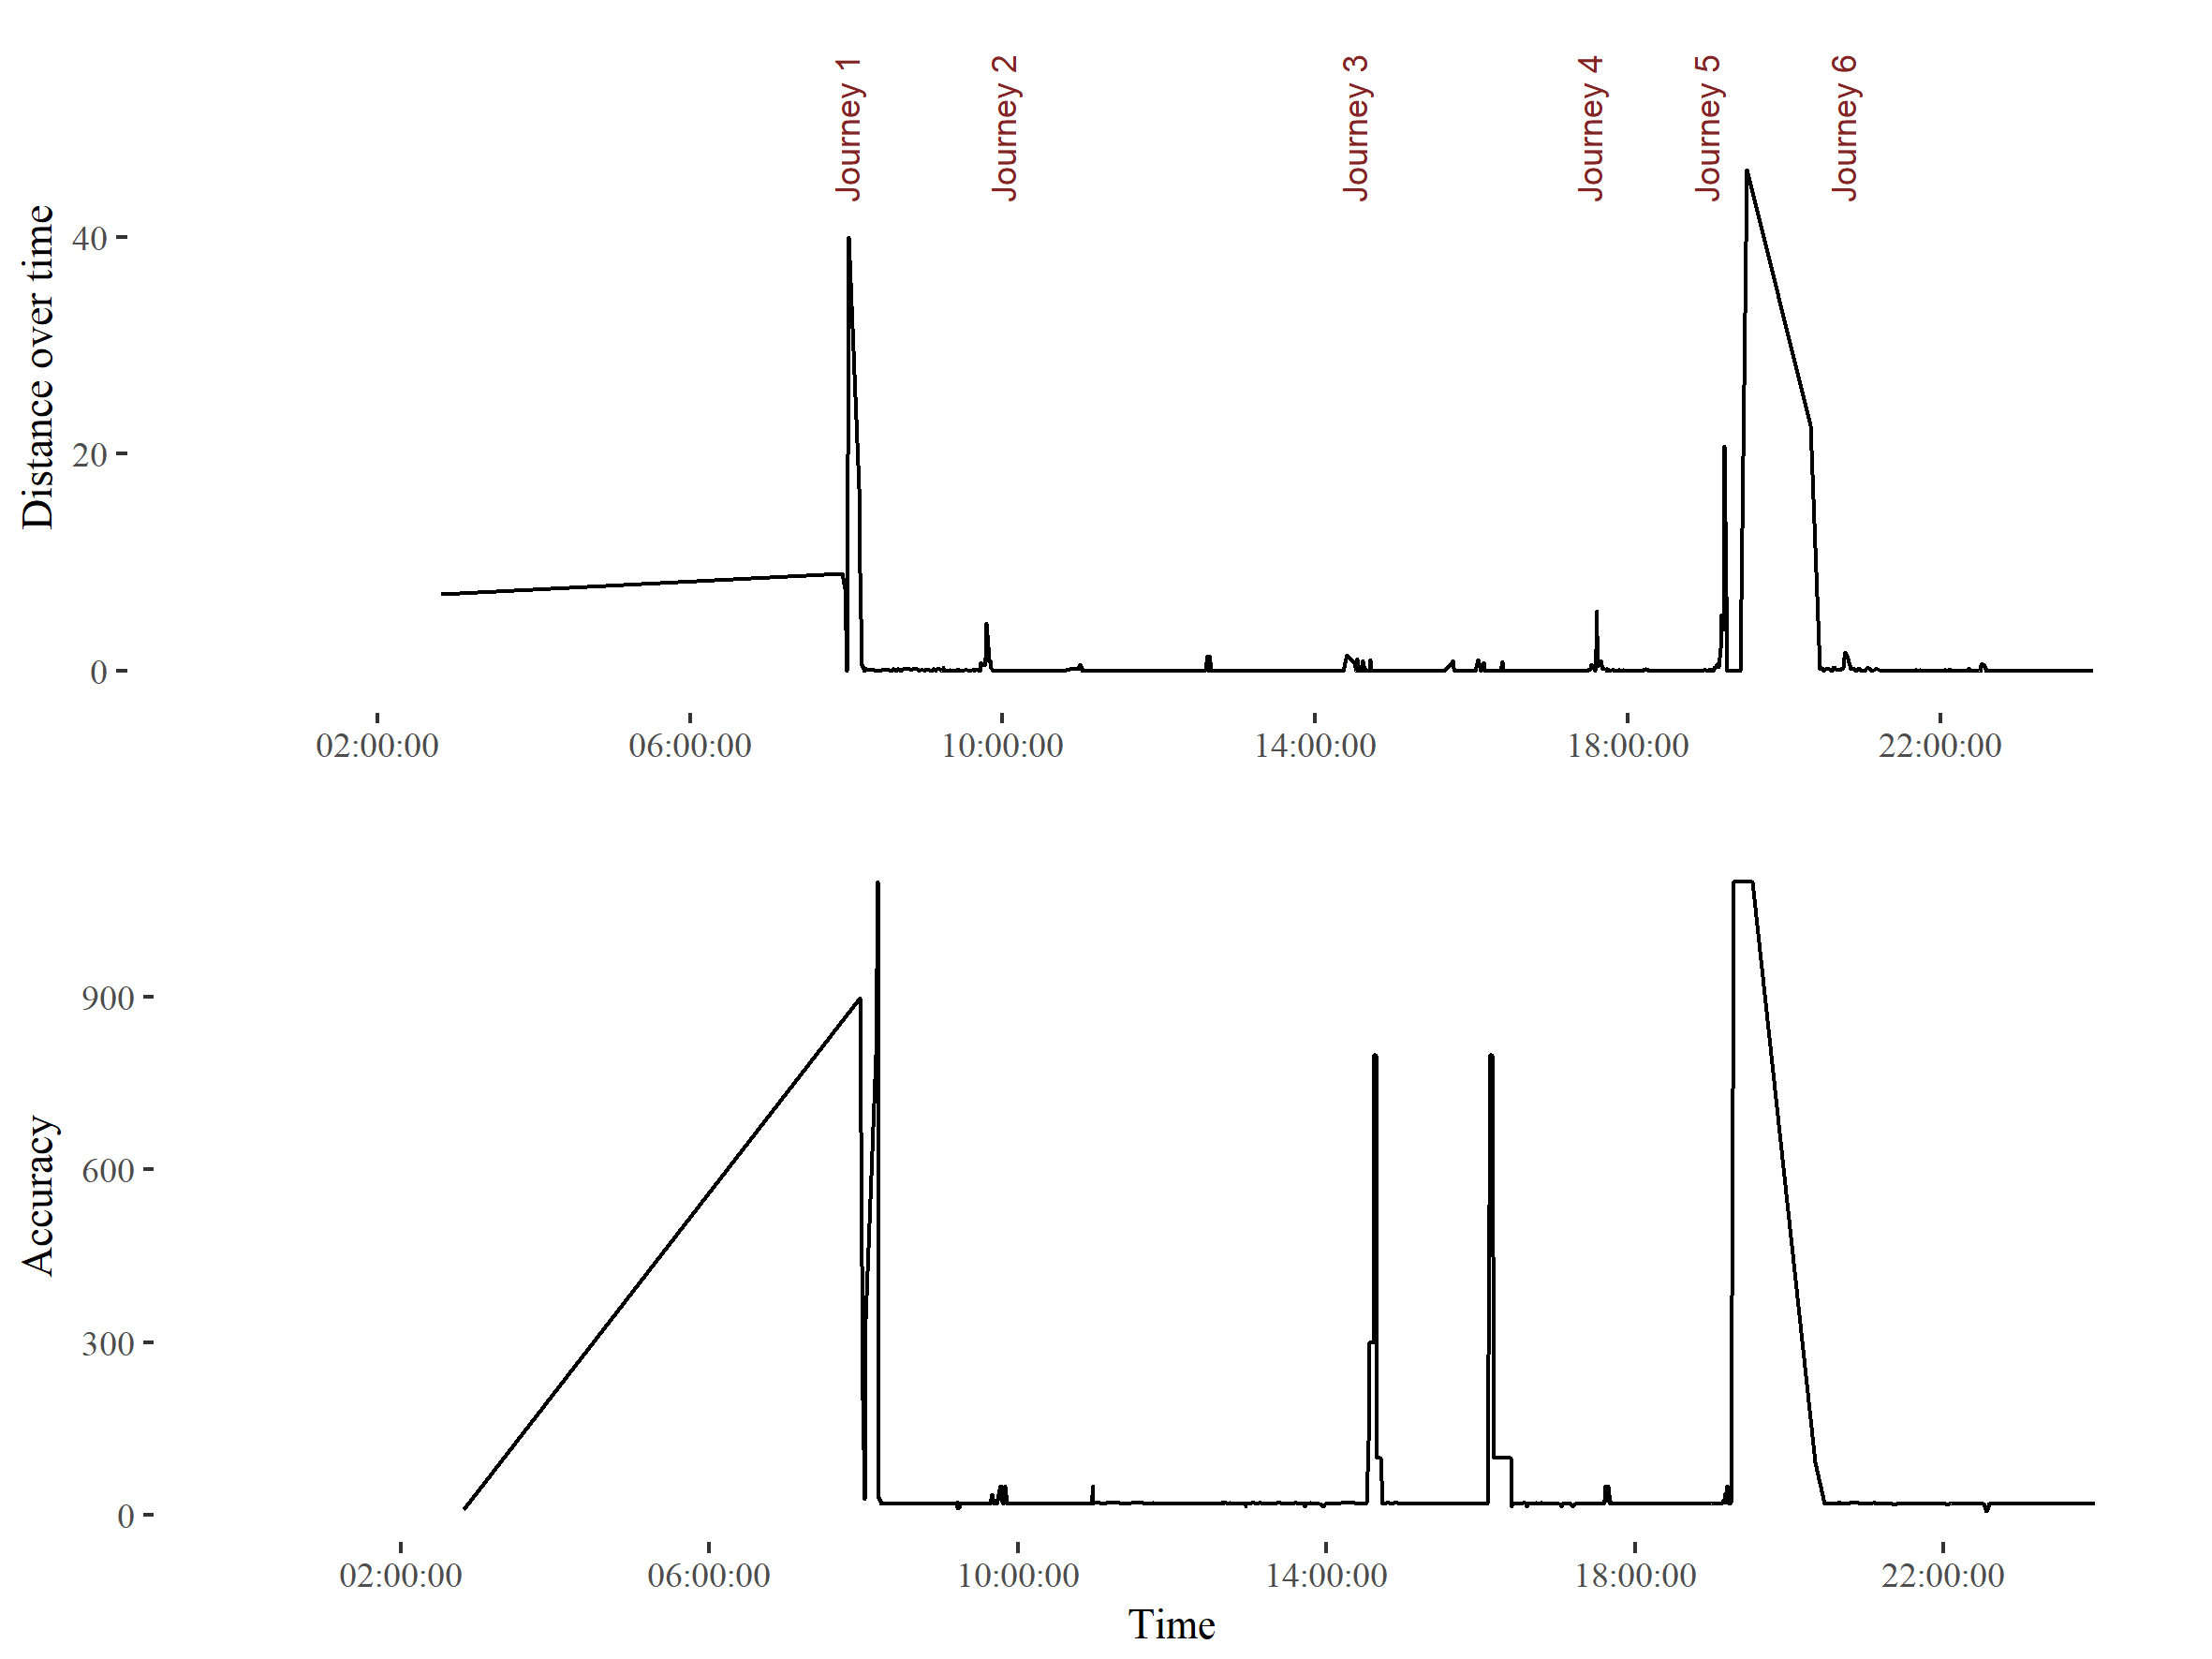
\includegraphics[width=1\linewidth]{img/accuracyLocShift} \caption{Measures of user activity and measurement accuracy on February 15th 2017.The upper chart shows the distance from the next measured point in meters over the course of the day. The first peak corresponds to the first journey from the user's home to a gym around 8am. The second, smaller peak before 10 reflects a journey from the gym to the nearby lecture theatre. Both journeys can be seen in Figure 1. The large jump between journey 5 and 6 is measurement error. The lower chart shows the accuracy over the course of the day. The figure shows that measurement inaccuracy is sometimes related to the movement of the individual. Stationary accuracy varies depending on phone battery level, wifi connection and user phone use.}\label{fig:accuracyPlot2}
\end{figure}

Noisy data can lead to inaccurate conclusions if it is not accounted
for. Suppose we wish to calculate an individual's movement in a day. A
simple approach would be to calculate the sum of the distance between
each measurement. But if there is noise, the coordinates will vary even
though the individual is not moving. If the measurements are frequent
and noisy, we will calculate a lot of movement, even if the individual
did not move at all! This issue is also visualised in Figure
\ref{fig:palmiusVme1}. The problem is further complicated because
missing data and noisy measurements are related. Methods used by
researchers to reduce noise, such as throwing out inaccurate
measurements (e.g. Palmius et al., 2017), can exacerbate the severity of
the missing data problem.

In this paper we will propose PPMI as a method for dealing with missing
data and measurement error in secondary location logs. We will compare
PPMI to similar solutions in the literature by evaluating the distance
between points which were simulated as missing and their imputed
counterparts. Finally we will calculate time spent at home as a function
of the imputation method.

\section{Related Work}\label{related-work}

How have researchers dealt with missing data in human mobility logs thus
far? Unfortunately there is no golden standard in how to deal with this
type of missing data. Researchers are generally vague about what
practices they follow (Jankowska et al., 2015). This vagueness is
worrisome as it invites solutions which contain significant researcher
degrees of freedom (Simmons, Nelson, \& Simonsohn, 2011). The vagueness
is possibly also due to the fact that most researchers are unfamiliar
with possible solutions. Most researchers simply down-sample temporally
and remove missing observations or use some sort of rule-based common
sense imputations (e.g. Palmius et al. (2017)). The only principled
approach that we know of that aims to solve the issue of missing data in
location logs as they relate to human mobility is that of Barnett and
Onnela (2016). We will explore the methods of Barnett and Onnela (2016)
and Palmius et al. (2017) in detail subsequently, after introducing
exploring other spatiotemporal methods.

A lack in methods for missing data imputation for human mobility
patterns does not imply there is not a vast literature on modelling
movement. The most widespread models are SSMs, therefore we shall detail
a few examples and subsequently argue that they are nonetheless unsuited
for long term human mobility logs. Ecologists have used SSMs to explain
how animals interact with their environment (Patterson, Thomas, Wilcox,
Ovaskainen, \& Matthiopoulos, 2008). These models can be quite complex.
Preisler, Ager, Johnson, and Kie (2004) uses Markovian movement
processes to characterise the effect of roads, food patches and streams
on cyclical elk movements. The most well studied SSM is the Kalman
filter, which is the optimal algorithm for inferring linear Gaussian
systems. The extended Kalman filter is the de facto standard for GPS
navigation (Z. Chen \& Brown, 2013). The advantage of state space models
is that they are flexible, deal with measurement inaccuracy, include
information from different sources and can be used in real time.

For secondary logs the main limitation of SSM implementations is that
they ignore movement routines. For instance, humans tend to go to work
on weekdays and sleep at night. Because SSMs are based on the Markov
property, they cannot incorporate this information. In other words, the
estimated location \(G(t)\) at time-point \(t\) is often based only upon
measurements \(D_t\), \(D_{t-1}\) and ignores all \(D_{t-i}|i\geq2\).
Hierarchical structuring and conditioning on a larger context have been
suggested as ways to add periodicity to Markovian models. These
solutions are often computationally intractable or unfeasible (Sadilek
\& Krumm, 2016). Moreover, these models often assume time and space
invariance (location is not a direct function of time or space). These
mathematical assumptions are violated in the case of human movement
patterns. For this reason we do not consider existing SSMs to be useful
for imputing missing data in this case.

In the wider realm of spatiotemporal statistics there are numerous
missing data imputation methods. These often come from climate or
geological research and rely on spatiotemporal auto-correlations. For
instance, the CUTOFF method estimates missing values by incorporating
similar observed temporal information from the value's nearest spatial
neighbors (Feng, Nowak, O'Neill, \& Welsh, 2014 ). The authors
illustrate their example using rainfall data from gauging stations
across Australia. Similarly, Z. Zhang et al. (2017) use a variety of
machine learning methods to impute missing values. The example provided
relates to underground water data. Generally these models assume fixed
measurement stations (such as rainfall gauging stations). For this
reason they cannot be easily applied to missing mobility tracks without
significant pre-processing.

On the other hand, a few researchers have explicitly attempted to impute
missing data from human mobility patterns ({\textbf{???}}; Barnett \&
Onnela, 2016; Palmius et al., 2017 ). Importantly, none of them worked
with secondary logs. Nonetheless we will detail what they did as
informative examples. Palmius et al. (2017) deal with the measurement
inaccuracy of \(D\) in custom logs by removing from the data set all
unique low-accuracy \(a\) data points that had
\(\frac{d}{dt}D > 100 \frac{km}{h}\). Subsequently the researchers down
sample the data to a sample rate of 12 per hour using a median filter.
Moreover, Palmius et al. (2017) explain:

\begin{quote}
\enquote{If the standard deviation of {[}\(D\){]} in both latitude and
longitude within a 1 h epoch was less than 0.01 km, then all samples
within the hour were set to the mean value of the recorded data,
otherwise a 5 min median filter window was applied to the recorded
latitude and longitude in the epoch}.
\end{quote}

Missing data was imputed using the mean of measurements close in time if
the participant was recorded within 500m of either end of a missing
section and the missing section had a length of \(\leq 2h\) or
\(\leq 12h\) after 9pm. In cases where the previous conditions are not
met no values are imputed.

Barnett and Onnela (2016) follow a different approach which is, to the
best of our knowledge, the only principled approach to dealing with
missing data in human mobility data. Barnett and Onnela (2016) work with
custom logs where location is measured for 2 minutes and subsequently
not measured for 10 minutes. In the words of the authors, Barnett and
Onnela (2016) handle missing data by first converting data to mobility
traces, which are defined as a sequence of flights and pauses. Flights
are segments of linear movements and pauses corresponding to periods of
time where a person does not move. Subsequently, the authors impute
missing data by:

\begin{quote}
\enquote{simulat{[}ing{]} flights and pauses over the period of
missingness where the direction, duration, and spatial length of each
flight, the fraction of flights versus the fraction of pauses, and the
duration of pauses are sampled from observed data.}
\end{quote}

This method can be extended to imputing the data based on temporally,
spatially or periodically close flights and pauses. In other words, for
a given missing period, the individual's mobility can be estimated based
on measured movements in that area, at that point in time or movements
in the last 24 hours (\emph{circadian proximity}).

On the other hand, ({\textbf{???}}) use what they call a Spatial
Temporal Semantic Neural Network (STS-NN) to predict future human
movement. While the authors are concerned with prediction and not
imputation, they devised a method called the Spatial Temporal Semantic
(STS) algorithm which converts raw measurements to machine learning
friendly discrete bins. Working with high-frequency measurements,
({\textbf{???}})'s method down-samples the raw data temporally and
map-matches the resulting bins to discrete points along pre-established
geographical features such as roads and highways. This minimises
measurement error and paves the way for applying machine learning
methods to human mobility problems.

In this section we have argued that there is a lack of established
practices to follow with respect to missing data in human mobility logs.
Moreover, extensively used spatiotemporal methods, such as state space
models (SSMs), are not well suited to deal with human mobility patterns
in secondary logs. Finally we discussed in detail three approaches which
deal explicitly with mobility patterns from custom or secondary logs
({\textbf{???}}; Barnett \& Onnela, 2016; Palmius et al., 2017 ).

\section{Methodology}\label{methodology}

\subsection{Notation}\label{notation}

Location measurements, such as those produced by GPS sensors, provide us
with coordinates (latitude and longitude) on the surface of the earth,
which is ellipsoid shaped. Projecting three dimensional measurements in
\(\mathbb{R}^3\) onto a two dimensional plane in \(\mathbb{R}^2\)
results in distortion. For clarity, when we use the term distance we
refer to the geodesic distances on an ellipsoid using the WGS84
ellipsoid parameters.

Subsequently let us simplify by assuming that a persons location is on
two-dimensional Euclidean plane. Let a person's true location on this
two-dimensional plane be \(G(t) = [G_x(t) G_y(t)]\) where \(G_x(t)\) and
\(G_y(t)\) denote the location of the individual at time \(t\) on the
x-axis and y-axis respectively. For simplicity, we can assume that the
x-axis is the longitude and the y-axis is the latitude. Moreover, let
\(D \in \mathbb{R}^2\) be the recorded data containing the latitude and
longitude. In addition, let \(a\) denote the estimated accuracy of the
recorded data. Furthermore, \(G(t)\), \(D\) and \(a\) are indexed by
time labeled by the countable set \(t = t_1 < ... < t_{n+1}\). The
measure of accuracy \(a_t\) is given in meters such that it represents
the radius of a 67\% confidence circle. If \(D_t = \emptyset\) it is
considered \emph{missing} and it is not missing otherwise.

When several data sets are available from individuals living in
overlapping areas we can construct a \(t \times i\) matrix \(M\) where
the entry \(M(t,i)\) contains \(G(t)\) for the individual \(i\).

\subsection{Personalised Map Matching
Imputation}\label{personalised-map-matching-imputation}

Our algorithm is designed to leverage the periodic nature of human
movement along with the long span of secondary to deal with measurement
sparsity and inaccuracy.

\paragraph{Modelling assumptions}\label{modelling-assumptions}

First, following Barnett and Onnela (2016) we categorise all time-points
\(t\) as either belonging to the set \(P\) (pause) or set \(F\)
(flight). Conceptually pauses can be understood as periods of time where
an individual spends significant amount of continuous time without
moving. Flights are the times where the individual is moving. Let
\(t_a\) be a pause of length \(n\). \[t_a = t_i < ... < t_{i+n}\] Let
\(t_b\) be a pause of length \(m\) such that there is no temporal
overlap between \(t_a\) and \(t_b\):
\[t_b = t_j= < ... < t_{j+m}|t_{i+n}< t_j\] Then it follows that between
the two pauses there must be a flight indexed by \(t_x\) of length
\(j-i+n\). \[t_x =  t_{i+n} < ... < t_{j} |t_x \in F\] We define pause
locations \(G(t_a), G(t_b) | t_a, t_b \in P\) as locations where an
individual spends an extended amount of time in the same space
(e.g.~school, home, work, train station, barber shop, bar, gym).
Importantly, our model assumes period and cyclic human movement such
that there are many pauses \(t_{a1},t_{a2},...,t_{an}\) such that
\(G(t_{a1}) = G(t_{a2}) = ... = G(t_{an})\). Moreover,it is possible for
\(G(t_a) = G(t_b)\) such that \(t_a \ne t_b\). For example, if the
individual leaves home for a run and returns home without stopping
anywhere else.

Let us define as \(Flight^x_{ab}\) the set of all points belonging to a
flight between \(G(t_a)\) and \(G(t_b)\) at time-point \(t_x\).
\[Flight^x_{ab}= G(t_x)|t_x \in F =  \{G(t_{i+n}),...,G(t_j)\}\] Again,
there are many flights \(t_{x1},t_{x2},...,t_{xn}\) such that
\(Flight^{x1}_{ab} = Flight^{x2}_{ab} = ... = Flight^{xn}_{ab}\). Then,
we can define as \(Path_{ab}\) the set of all flights between \(G(t_a)\)
and \(G(t_b)\) at all time-points. For simplicity, we assume that
\(Path_{ab}=Path_{ba}\).

In addition, we consider all measurements \(D(t)\) to be imperfect
measurements of \(G(t)\):

\[ G(t) = D(t) + \text{Measurement Error}  \]

\subsection{Personalised Map Matching Imputation
algorithm}\label{personalised-map-matching-imputation-algorithm}

Our algorithm performs the following steps:

\begin{enumerate}
\def\labelenumi{\arabic{enumi}.}
\tightlist
\item
  \emph{Map building}: Extract from measurements \(D\) all pause
  location bins and path location bins to create a personalised map.
\item
  \emph{Binning}: Assign each measurement \(D\) to a unique discrete
  location bin.
\item
  \emph{Imputing}: Use a classification method to predict missing
  measurements based on all the available information.
\end{enumerate}

\subsubsection{Map building}\label{map-building}

Following ({\textbf{???}})'s spatial-temporal-semantic (STS) feature
extraction algorithm our aim is to transform pause and path locations
into machine learning friendly discrete location sequences. There are
multiple ways of extracting such measurement clusters in the literature,
such as Spatio-Temporal Density-Based Spatial Clustering of Applications
with Noise (ST-DBSCAN) and sequence oriented clustering (SOC)
{[}(``ST-DBSCAN,'' 2007);{]}. We will focus on two methods which
explicitly with mobility patterns from unevenly sampled smartphone logs
(Barnett \& Onnela, 2016; Palmius et al., 2017 ). Both of these methods
pre-process the data and subsequently use two steps to extract pause
locations: first they extract pauses and their corresponding locations,
then they cluster pause locations based on spatial proximity. This
implementation of PMMI uses a stricter version of Barnett and Onnela
(2016)'s approach to extract pauses.

First the measurements \(D\) are filtered such that only measurements
with an accuracy value lower than \(a_{\text{P lim}}\) remain within the
sample. Then, a measurement \(D_t\) belongs to a pause if and only if:

\begin{enumerate}
\def\labelenumi{\arabic{enumi}.}
\tightlist
\item
  The next measurement \(D_{t+1}\) is within \(t_{\text{Pause lim}}\)
  amount of seconds (so it is not missing)
\item
  The next measurement \(D_{t+1}\) is within \(d_{\text{Pause lim}}\)
  meters.
\item
  The duration of the pause is more than \(\delta_{\text{Pause lim}}\)
  seconds.
\item
  Let the measurements of a possible pause which fit the aforementioned
  criteria be \(D_{t,t+1,...,t+n}\). These points are only a pause if
  the distance between the mean coordinates of \(D_{t,t+1,...,t+n}\) and
  the furthest away points of \(D_{t,t+1,...,t+n}\) is within 2 times
  the mean accuracy \(a\) of \(D_{t,t+1,...,t+n}\).
\end{enumerate}

This set of points were then hierarchically clustered using a distance
matrix, such that all points within \(d\) meters of each other were
clustered into a pause location. Each pause location is a bin.

For all remaining measurements we assume that they belong to paths. In
this implementation of PMMI we use the following algorithm to estimate
paths:

\begin{enumerate}
\def\labelenumi{\arabic{enumi}.}
\tightlist
\item
  Take all measurements which are not pauses, filter them based on an
  accuracy threshold \(a_{\text{Path Lim}}\).
\item
  Create a distance matrix for all remaining measurements \(D_t \in F\)
  and hierarchically cluster it accordingly, such that all points within
  \(d_{\text{Path Lim}}\) meters of each other are clustered into a
  single pause point.
\end{enumerate}

At this point all empirically observed path bins and pause bins are
extracted. However, there may be some overlap between pause bins and
path bins. Thus, the bins are clustered again, such that the pause bins
retain priority. This means that if a pause bin and a path bin are
within less than \(d\) meters of each other, the path bin is removed.
The reasoning for this is that the threshold for not being in a pause
cluster should be higher, as individuals spend the majority of time at a
pause cluster. The end result is a discretised map which contains pause
and flight bins based on the entire log history of the individual.

\subsubsection{Binning}\label{binning}

({\textbf{???}})'s spatial-temporal-semantic (STS) feature extraction
algorithm uses map matching as a ground truth to assign noisy
measurements into discrete bins along roads. In other words, in addition
to the measured data they also use a geographic database that contains
information about the area in which the individual is (e.g.~where
precisely the roads are), and sort measurements into bins based on both
the measurement and the geographic data base. For example, if an
individual is measured as moving closely in parallel to a road A in an
area where there is no other parallel road, ({\textbf{???}})'s method
will assume that the individual is on the road A.

PMMI uses a similar logic, but without using any external geographic
database. The key modification in PMMI is that whilst ({\textbf{???}})
uses a map from outside the persons location logs, we use the total
location history of the individual to create a personalised map. This
map is subsequently used to bin measurements. This is feasible for two
reasons: humans tend to have repetitive movement habits and secondary
logs tend to be long. To put it in simpler terms, we consider each
measurement at \(D_x\) as a sample of \(Path_{ab}\), and by aggregating
many measurements we can use them to map out \(Path_{ab}\).

Thus, all measurements \(D\) were are then assigned to a discrete bin on
the personal map. This includes previous measurements which were
discarded from the map building exercise due to an accuracy \(a\) value
which exceeded \(a_{\text{P lim}}\) or \(a_{\text{F lim}}\). In this
implementation we used a simple assigning function, whereby the
measurements where assigned to the bin nearest to the measurement.

\subsubsection{Classification}\label{classification}

At this point the objective of PMMI is to take all the information
available about the mobility history of an individual and impute the
missing value. In this implementation we trained an artificial neural
network (ANN) to do so. For more information on the precise architecture
of the artificial neural network please consult the appendix. The input
variables to the ANN are:

\begin{enumerate}
\def\labelenumi{\arabic{enumi}.}
\tightlist
\item
  The previous and subsequent observed bin as a binary class matrix.
\item
  The distance in time to the next \& previous bin.
\item
  The time of the day encoded as a cyclical two-dimensional feature.
\item
  The day of the month as a binary class matrix.
\item
  The month of the year as a binary class matrix.
\end{enumerate}

For the encoding of the time of day we took the cosine and the sine
transforms of the amount of seconds that have elapsed after midnight
(London, 2016). This is necessary so that the model can understand that
one second past midnight and one second before midnight are in fact two
seconds away from each other. Moreover we scaled the non-binary values
to occupy a range between 0 and 1 in order to ensure convergence.

For a missing time-point at \(D_t \in \emptyset\), the output of the
model is a set of probability estimates associated with every location
cluster. That is, for each missing time-point the model returns a vector
of probability estimates (with one estimate per bin) associated with
where the individual is.

\subsection{Datasets \& Analyses}\label{datasets-analyses}

The secondary location log used to train the imputation methods was
collected between 2013 and 2017 on different Android devices from a
single individual. About 54\% of the data is missing for the entire
duration of the log. This may be misleading as there are several long
periods with no measurements whatsoever. For days which were not
entirely missing, approximately 22\% of all five minute segments were
missing. The structure of missingness of a day with measurements is
shown in Figure \ref{fig:measurementsPerDay}. As you can see, there are
several long periods over the course of the log for which there are no
measurements. The median sampling frequency per day for non-missing days
is around 0.006 Hz.

\begin{figure}
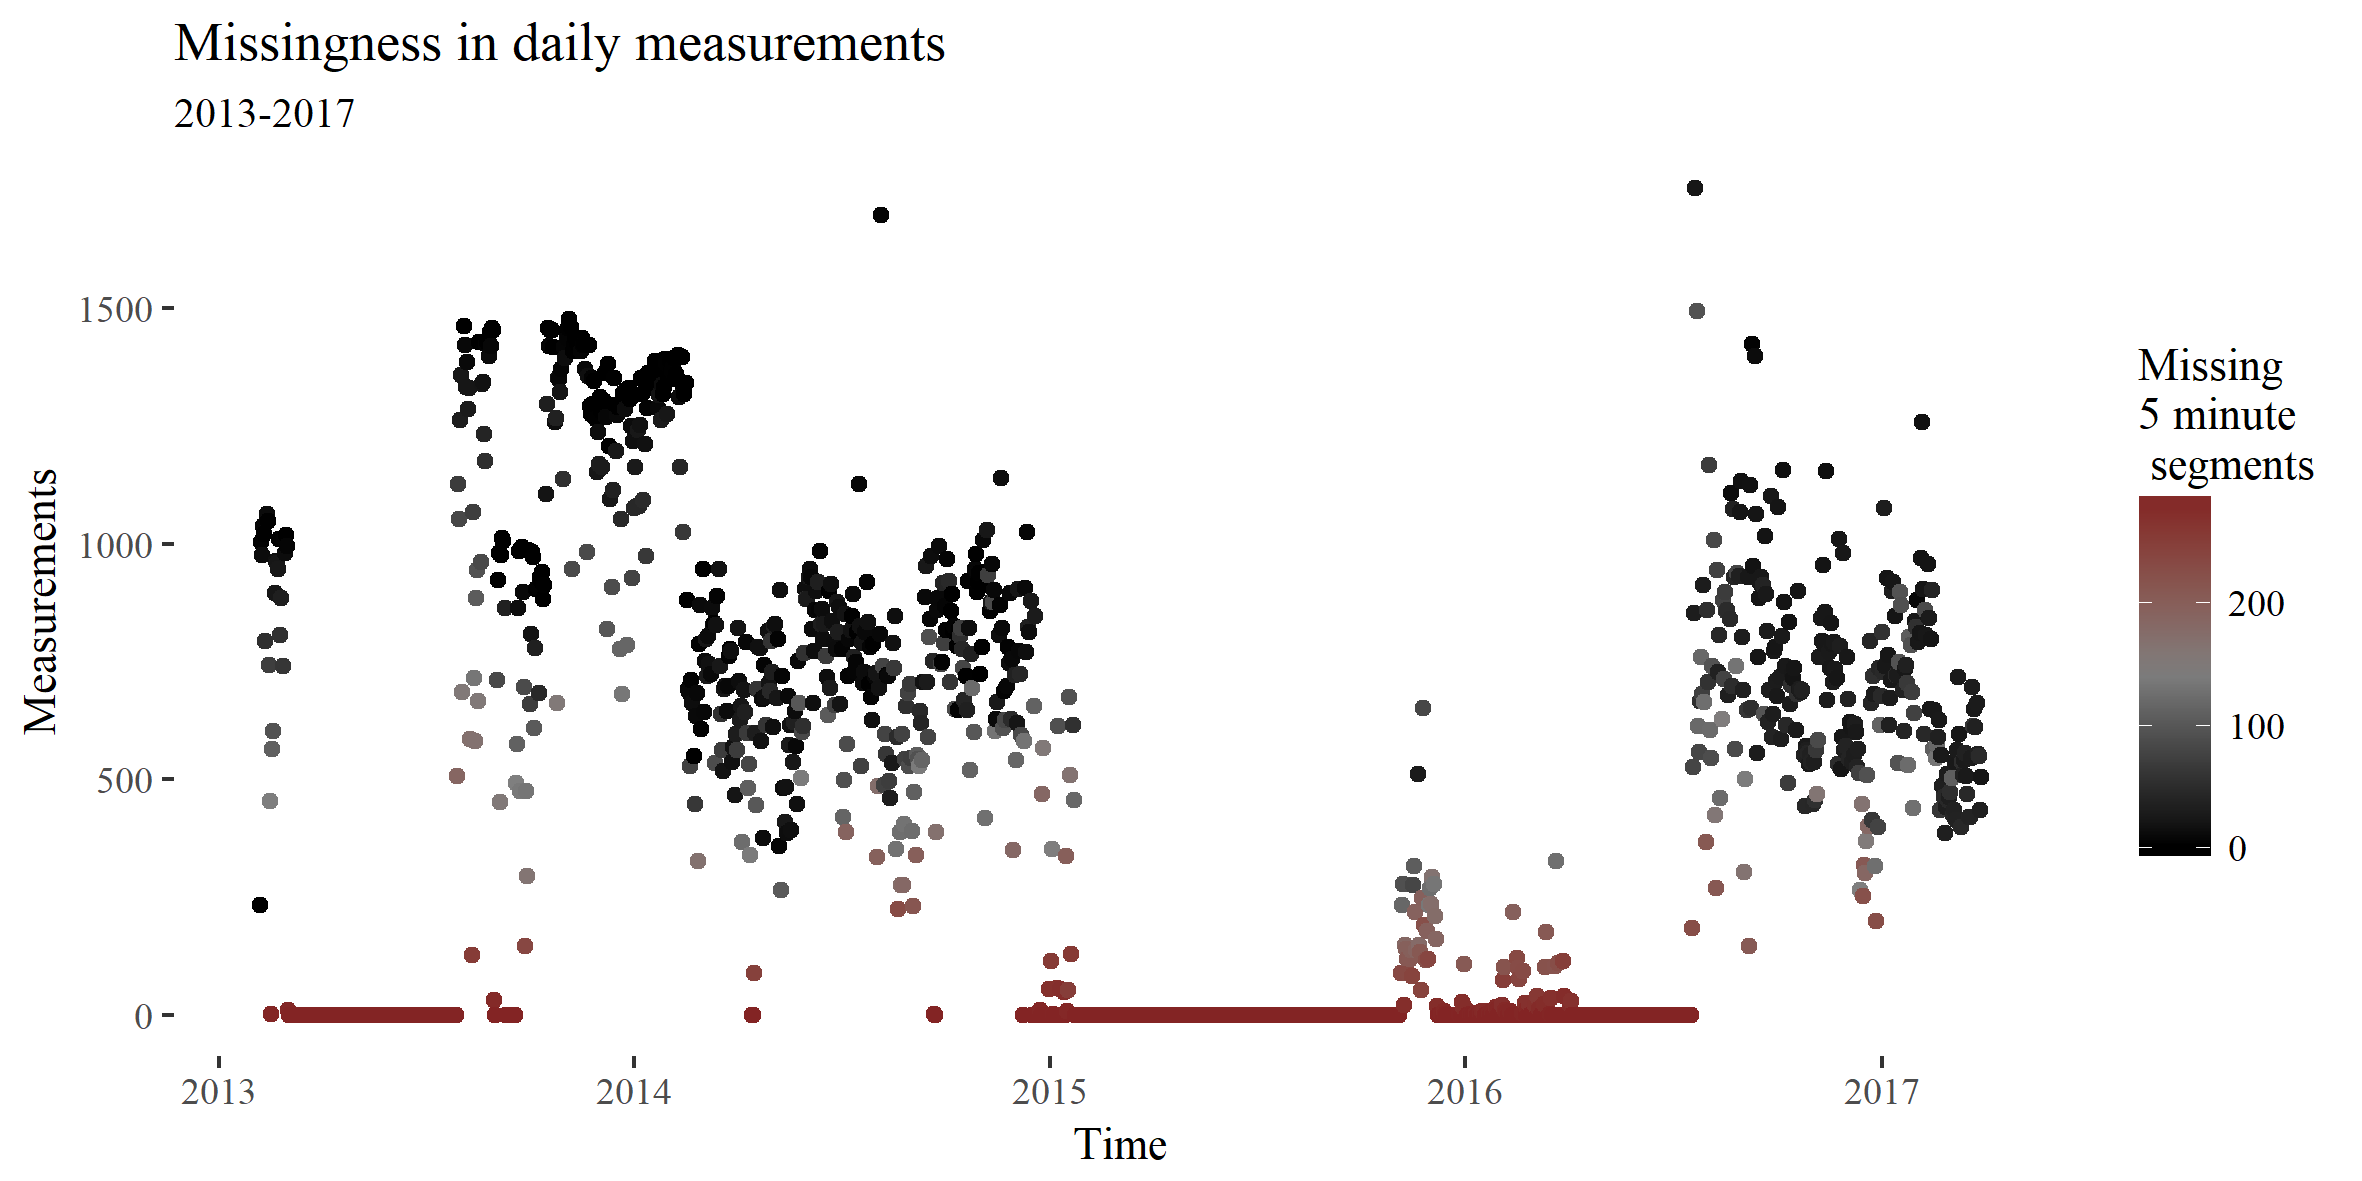
\includegraphics[width=1\linewidth]{img/missingdayBoaz5min} \caption{Missing data for the entire duration of the log. The x-axis denotes time, the y-axis shows how many measurements are made and each point is a five minute window. For this day there were several periods with no information. These points are filled with red and lie on the x-axis.}\label{fig:measurementsPerDay}
\end{figure}

For simplicity, we subsequently used a time period when the individual
was living in the Netherlands. This leaves us with 156,000 measurements
over a period of less than six months. Analyses as well as
implementations and adaptions Palmius et al. (2017)'s and Barnett and
Onnela (2016)'s model were performed using R and a multitude of other
statistical packages R (Version 3.4.3; R Core Team, 2017) and the
R-packages \emph{ggplot2} (Version 2.2.1; Wickham, 2009),
\emph{ggthemes} (Version 3.4.0; Arnold, 2017), \emph{knitr} (Version
1.20; Xie, 2015), and \emph{papaja} (Version 0.1.0.9709; Aust \& Barth,
2018). All the code is available on a public repository
({\textbf{???}}).

\subsection{Results \& Evaluation
Metrics}\label{results-evaluation-metrics}

The results will consist of multiple steps:

\begin{enumerate}
\def\labelenumi{\arabic{enumi}.}
\tightlist
\item
  Evaluating the performance of the map building and assigning
  functions.
\item
  Comparing the performance of PMMI using a) baseline models b)
  performance with randomly removed data in comparison to the
  aforementioned methods (Barnett \& Onnela, 2016; Palmius et al., 2017)
  and c) objective ground-truth data (public transportation
  time-stamps).
\end{enumerate}

\subsubsection{Map building \& binning
evaluation}\label{map-building-binning-evaluation}

Before we can evaluate the accuracy of the imputations, it is essential
to evaluate how well noise in the data has been cleaned. Otherwise we
run the risk of over-fitting the model in the sense that we will measure
the extent to which an imputation method can correctly impute
measurement noise within \(D_t\) instead of true location \(G(t)\).

In order to evaluate the map building and binning we will first visually
evaluate the paths and pause locations. A visual evaluation of paths
superimposed on is an established way to heuristically check their
accuracy (e.g. ({\textbf{???}})). Then, let the average distance between
the actual measured point and the binned point be the \emph{deviation
distance} \(\delta_{\text{dev}}\). With respect to the deviation
distance \(\delta_{\text{dev}}\), we expect:

\begin{enumerate}
\def\labelenumi{\arabic{enumi}.}
\tightlist
\item
  A positive relationship between the deviation distance and the
  accuracy of each measurement.
\item
  Roughly 67\% of the deviation distances \(\delta_{\text{dev}}\) are
  within accuracy \(a\) of each measurement.
\end{enumerate}

\subsubsection{Imputation algorithm
performance}\label{imputation-algorithm-performance}

We will compare the performance of PMMI, Palmius et al. (2017) and
Barnett and Onnela (2016). In addition, we will also compute a naive
model, which simply imputes as the missing value the previous observed
value. The naive model will serve as a baseline model. To compare the
performance of these methods we will remove 25\% of measured time
intervals at random within a four week period. We will make our
comparisons for intervals of 5 minutes, 1 hour and 1 day. In other
words, we will remove 25\% of time intervals at random, while varying
the size of the time intervals removed.

For the Barnett and Onnela (2016) and PMMI models we will use all the
available data to train the models with the exception of the time
periods being investigated. Palmius et al. (2017)'s model does not
require training.

To compare all methods with each other we will compute a distance
measure (how far was the removed location from the predicted location).
For PMMI's imputations we will use a weighted mean for the distance
measures whereby each 5 minute period is weighted equally. This is
necessary because the other two model estimate far fewer values than
PMMI. While Barnett and Onnela (2016)'s and Palmius et al. (2017)'s
models estimate 12 measurements for each missing hour, PMMI estimates as
many measurements as there are in the log. When individuals go to
infrequently travelled locations they tend to use their phone's location
services more than 100 more times, which leads to more measurements, and
hence more imputed values. Hence, if the weights are not used PMMI is
susceptible to error overestimates which are related to measurement
frequency in a way that the other two methods are not.

In addition, other measures of interest for PMMI are accuracy (in what
percentage of the cases was the appropriate cluster predicted), the
\emph{confidence} and the \emph{distance expectation}. The confidence is
the probability with which the model predicts the most likely cluster.
For instance, if the model predicts the missing bin to be bin A with a
probability of 0.9 then we can say it has high confidence in the
prediction. Similarly, the distance expectation is the cross-product of
the estimated probabilities that the individual is at any of all given
clusters and the distances between the clusters to the true cluster. For
example, if the true location of an individual is bin A (bin A is 10
meters away from bin B) and the model assigns a probability of 0.9 at
bin A and 0.1 at bin B, then the distance expectation would be 1 meter.

Finally, we will take objective real world data and compare it to
predicted values. We will use information from the Dutch public
transportation card. The Dutch public transportation service provides
users with time-stamped data of when and where they board, change lines
or leave public transportation. To be able to make a comparison between
models we will remove all measurements from within the 5 minute period
that a time-stamped measurement is available. Then we will use each
model to impute the location of the individual within that period.

\section{Results}\label{results}

\subsection{Map building \& binning
evaluation}\label{map-building-binning-evaluation-1}

We used the following parameters to extract pauses: an accuracy limit
\(a_{\text{Pause lim}}\) of 250 meters, a time limit
\(t_{\text{Pause lim}}\) of 300 seconds, a distance limit of
\(d_{\text{Pause lim}}\) 50 meters and a minimum pause duration limit
\(\delta_{\text{Pause lim}}\) of 100 seconds. Moreover, to extract path
clusters we used the parameters:
\(a_{\text{Path Lim}} = 150 \text{meters}\) and
\(d_{\text{Path Lim}} =300 \text{meters}\).

The selection of these parameters was more-or-less heuristically driven
based on their on their ability to extract a meaningful personalised
map. When selecting parameters there is a trade off is between bias and
precision. This is because an increase in precision in the form of a
higher for high density locations resolution comes at the expense of
precision as assigning measurements to bins becomes more difficult. For
instance, by increasing the clustering distance parameter
\(d_{\text{Pause lim}}\) we can extract more valid pause locations at
the expense of falsely categorising certain measurements to the wrong
cluster. This is illustrated in Figure \ref{fig:pauseLocUithof1}.

\begin{figure}
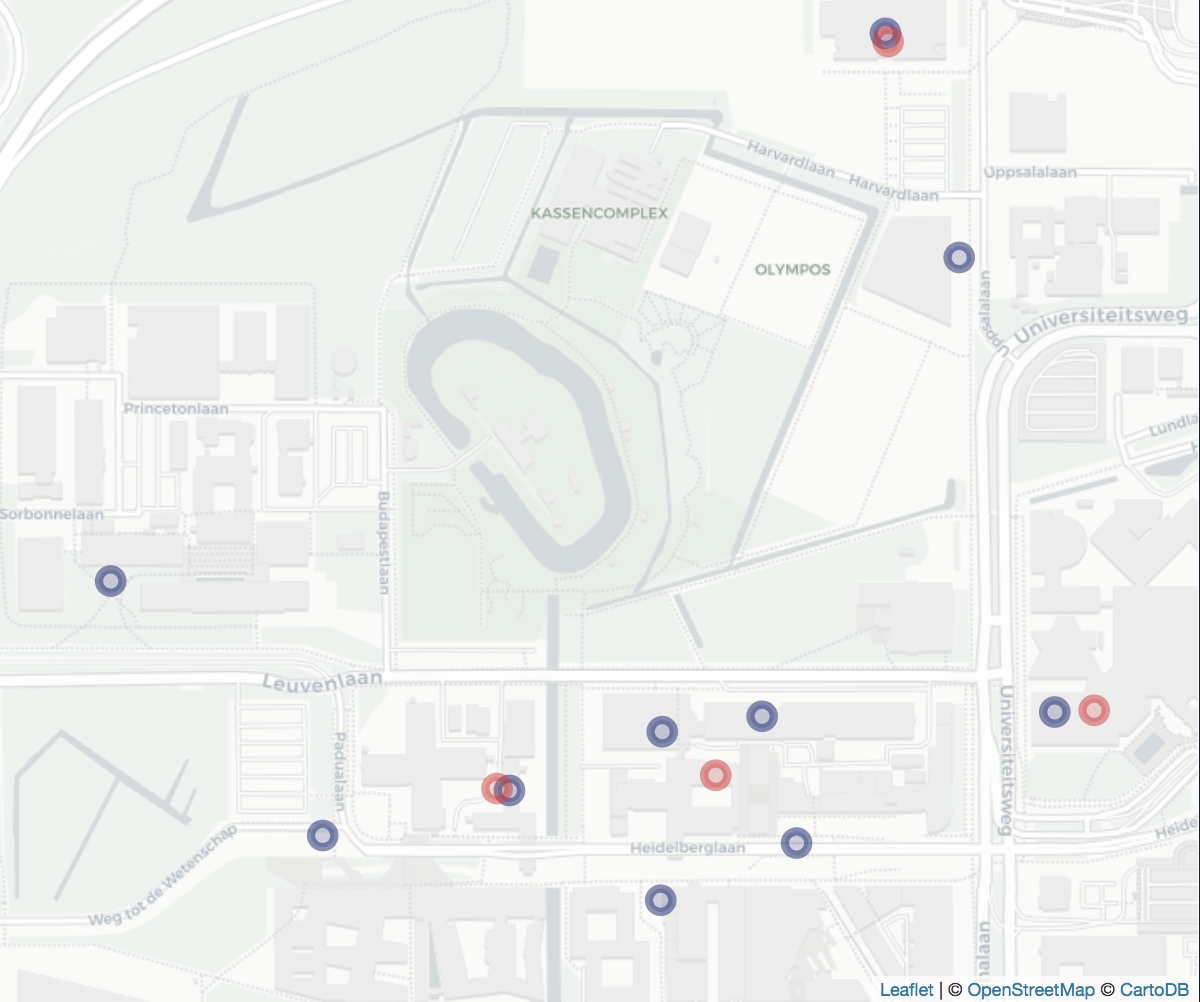
\includegraphics[width=1\linewidth]{img/distanceParam} \caption{Example of pause locations in De Uithof university campus using 150 meters (blue) and 400 meters (red) as clustering parameters.}\label{fig:pauseLocUithof1}
\end{figure}

Map building results in a personalised map with pause and path clusters.
An excerpt can be seen in Figure \ref{fig:mapClusterMap}. It is
important to remind the reader that PMMI is map agnostic and uses no
information from the map. Therefore, the close overlap with features on
the map, such as pause bins at relevant buildings and transportation
clusters, as well as the flight bins following roads and railway lines
indicate a high degree of precision in personal map building. As
expected, PMMI's path extraction yields greater accuracy for frequently
occurring paths. For example, the frequently travelled Amsterdam-Utrecht
railway line has been extracted almost perfectly, while the less
frequently travelled Utrecht-Enschede line is far sparser.

\begin{figure}
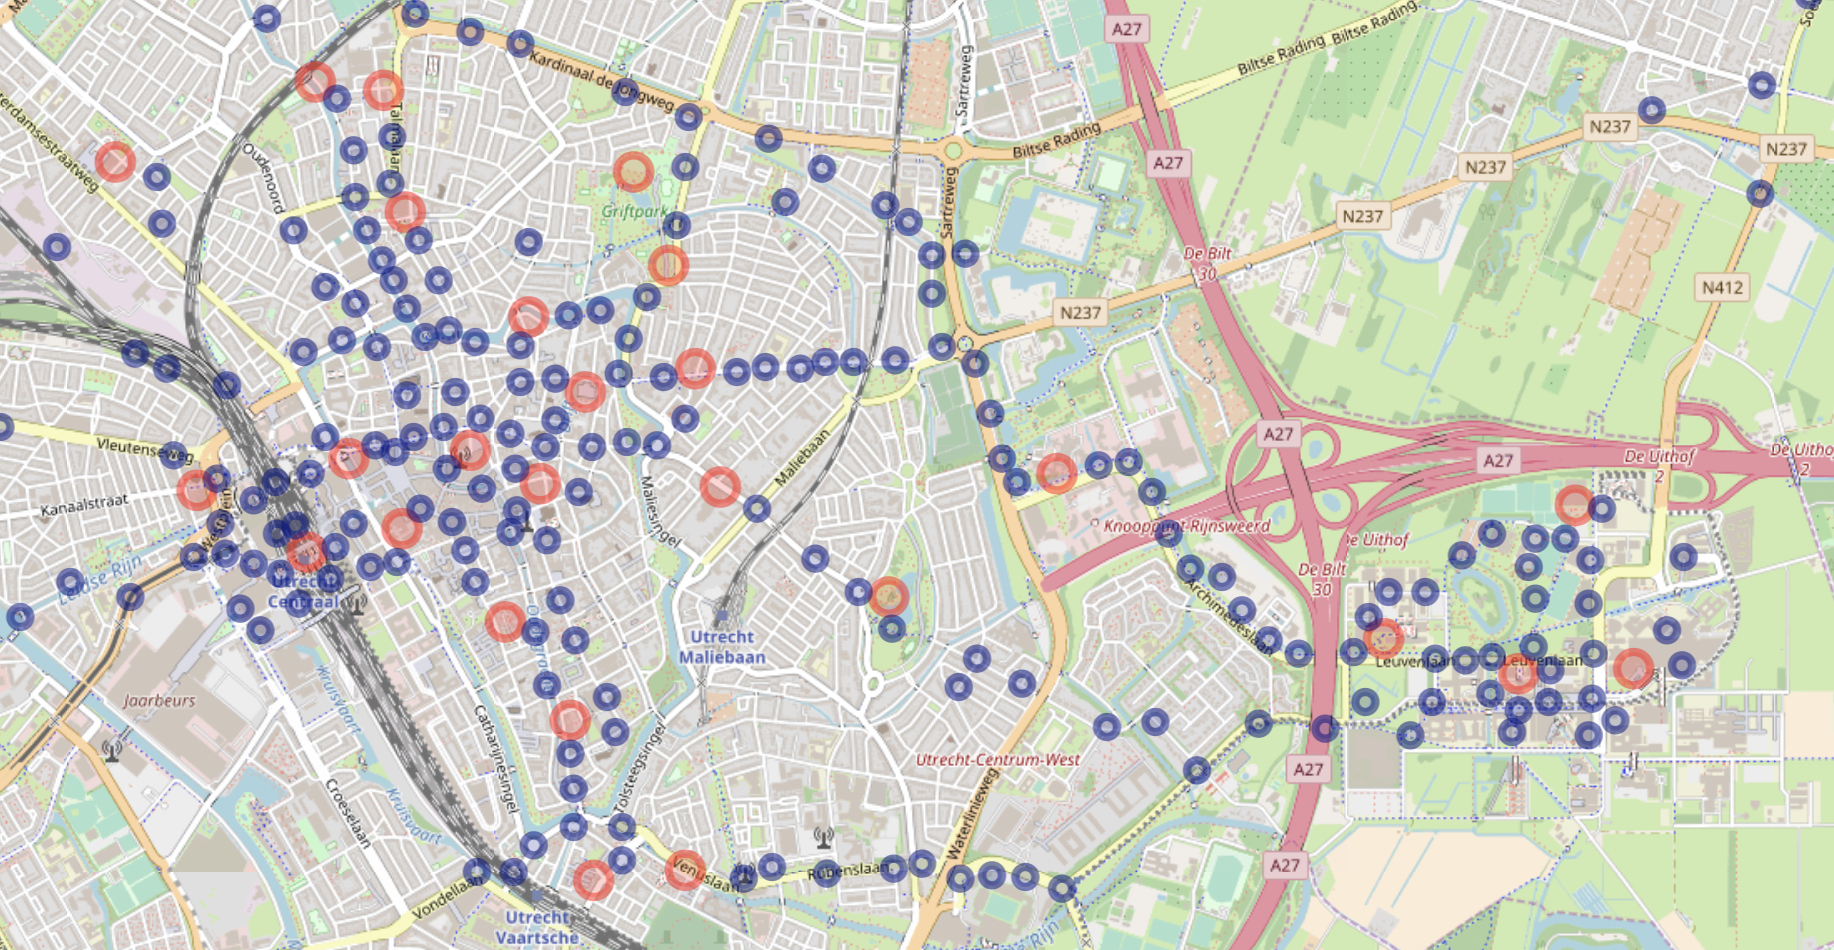
\includegraphics[width=1\linewidth]{img/mapClusterMap} \caption{Excerpt of the cluster map of an individual. Red points are pause locations, blue points are path locations.}\label{fig:mapClusterMap}
\end{figure}

For the entire period examined period the we find a deviance of 40
meters and a median deviance of 15 meters. Around 69\% of the deviance
values are within their corresponding accuracy value, which is close to
the theoretical \(\frac{2}{3}\) value that is expected. Approximately
9\% of values were not taken into account when creating the bins,given
that their the accuracy \(a\) exceeded \(a_{\text{Path Lim}}\).

For the narrower period of March 2017 approximately 74\% of the deviance
values are within their corresponding accuracy values, which is close to
the theoretical \(\frac{2}{3}\) value that is expected. The raw
unweighted mean and median deviance are 38 and 14 meters respectively.
If we weight them such that each 5 minute interval is weighted equally
to ease comparison with the other two methods, we find a mean deviance
of 35 meters with a median of 12.8.

In comparison, Palmius' method has a median deviance
\(\delta_{\text{dev}}\) of 3 meters, with a mean of 115 due to high
deviance outliers. On the other hand, Barnett's method has mean deviance
\(\delta_{\text{dev}}\) of 343 meters and a median deviance of 8 meters.
Barnett's deviance is necessarily higher than Palmius', as they
down-sample temporally (like Palmius) and subsequently aggregate into
pauses and linear flights.

The key difference between temporal and spatial down-sampling is shown
in Figure \ref{fig:palmiusVme1}. Temporal down-sampling is much more
sensitive to noise in sparsely measured periods because it averages out
values within five minute periods. Often there are only a few noisy
measurements in those periods (see Figure
\ref{fig:longMeasurementsPerDay} ), which leads to a noise in the
down-sampled values. Unsurprisingly, there is a positive relationship
between deviance and the amount of measurements in each down-sampled
interval. The fact that over 90\% of deviance values are within accuracy
(much higher than the expected theoretical 67\%) confirms that temporal
down-sampling is not sufficiently filtering out the noise.

\begin{figure}
\includegraphics[width=1\linewidth]{img/tempVsspace} \caption{Excerpt. MISSING CAPTION HERE}\label{fig:palmiusVsMe1}
\end{figure}

\subsubsection{Imputation evaluation}\label{imputation-evaluation}

The Palmius et al. (2017) model failed to impute 3\% of all removed
values for both the 5 minute and over 10\% for the 1 hour tests. Palmius
et al. (2017)' model failed to impute a single value for the day tests.
Similarly, Barnett and Onnela (2016)'s method failed to impute over 11\%
of the missing values. PPMI made an imputation for all missing values.
Table 1 shows the results of the distance metrics for each method.

\begin{table}[htb]
\begin{center}
\begin{threeparttable}
\caption{\label{tab:resulttable}Distance in meters between the removed time period and the imputed value.}
\begin{tabular}{lllllll}
\toprule
 & \multicolumn{2}{c}{Five minutes} & \multicolumn{2}{c}{One Hour} & \multicolumn{2}{c}{One Day} \\
\cmidrule(r){2-3} \cmidrule(r){4-5} \cmidrule(r){6-7}
 & \multicolumn{1}{c}{Mean} & \multicolumn{1}{c}{Median} & \multicolumn{1}{c}{Mean} & \multicolumn{1}{c}{Median} & \multicolumn{1}{c}{Mean} & \multicolumn{1}{c}{Median}\\
\midrule
Barnett \& Onella & 82 & 4 & 345 & 6 & 9,273 & 12\\
Palmius & 43 & 0 & 497 & 4 & NA & NA\\
PPMI & 269 & 0 & 908 & 0 & 5,757 & 0\\
Naive Baseline & 426 & 0 & 1,502 & 0 & 14,266 & 1,288\\
\bottomrule
\end{tabular}
\end{threeparttable}
\end{center}
\end{table}

In terms of PPMI's accuracy in this period, the prediction accuracy was
88\%, 73\% and 47\% for the 5 minute, 1 hour and 1 day periods
respectively. As a comparison, the naive model's accuracy ratings were
87\%, 68\% and 24\% respectively. The distance expectation values were
very similar to the distance scores, albeit approximately 5\% higher.
Confidence scores ranged from 0.006 to 1.

\subsubsection{Comparison with objective
data}\label{comparison-with-objective-data}

Once we removed the measurements within the 5 minute period of each
time-stamp, we employed the models to predict the location of the
individual at the time-stamped period. The naive model reaches an
accuracy of 16\%, with a median distance of 555 meters and mean distance
of 3303 meters. On the other hand MYMETHOD has an accuracy of 24\%, with
a median distance of 1037 meters and a mean distance of 5637. Again the
expectation of the distance was quite similar to the distance with a
mean of 6432 and a median of 1037 meters.

Palmius's model failed to impute 38 out of 97 periods. For those it did
impute, it showed a mean distance of 1517 meters and a median distance
of 1617. Barnett's model failed to impute 18 out of 97 periods. For
those it did impute, it had a mean of 5506 and a median of 1342.

\subsubsection{Example: effect on aggregate
measures}\label{example-effect-on-aggregate-measures}

Social scientists are most interested in aggregating spatiotemporal data
to more socially relevant information, such as the amount of time spent
at home. As an example we calculated the time spent at home of the user
in the month of March (Figure \ref{fig:aggrePlot}) without any model and
with all three of the investigated methods.

\begin{figure}
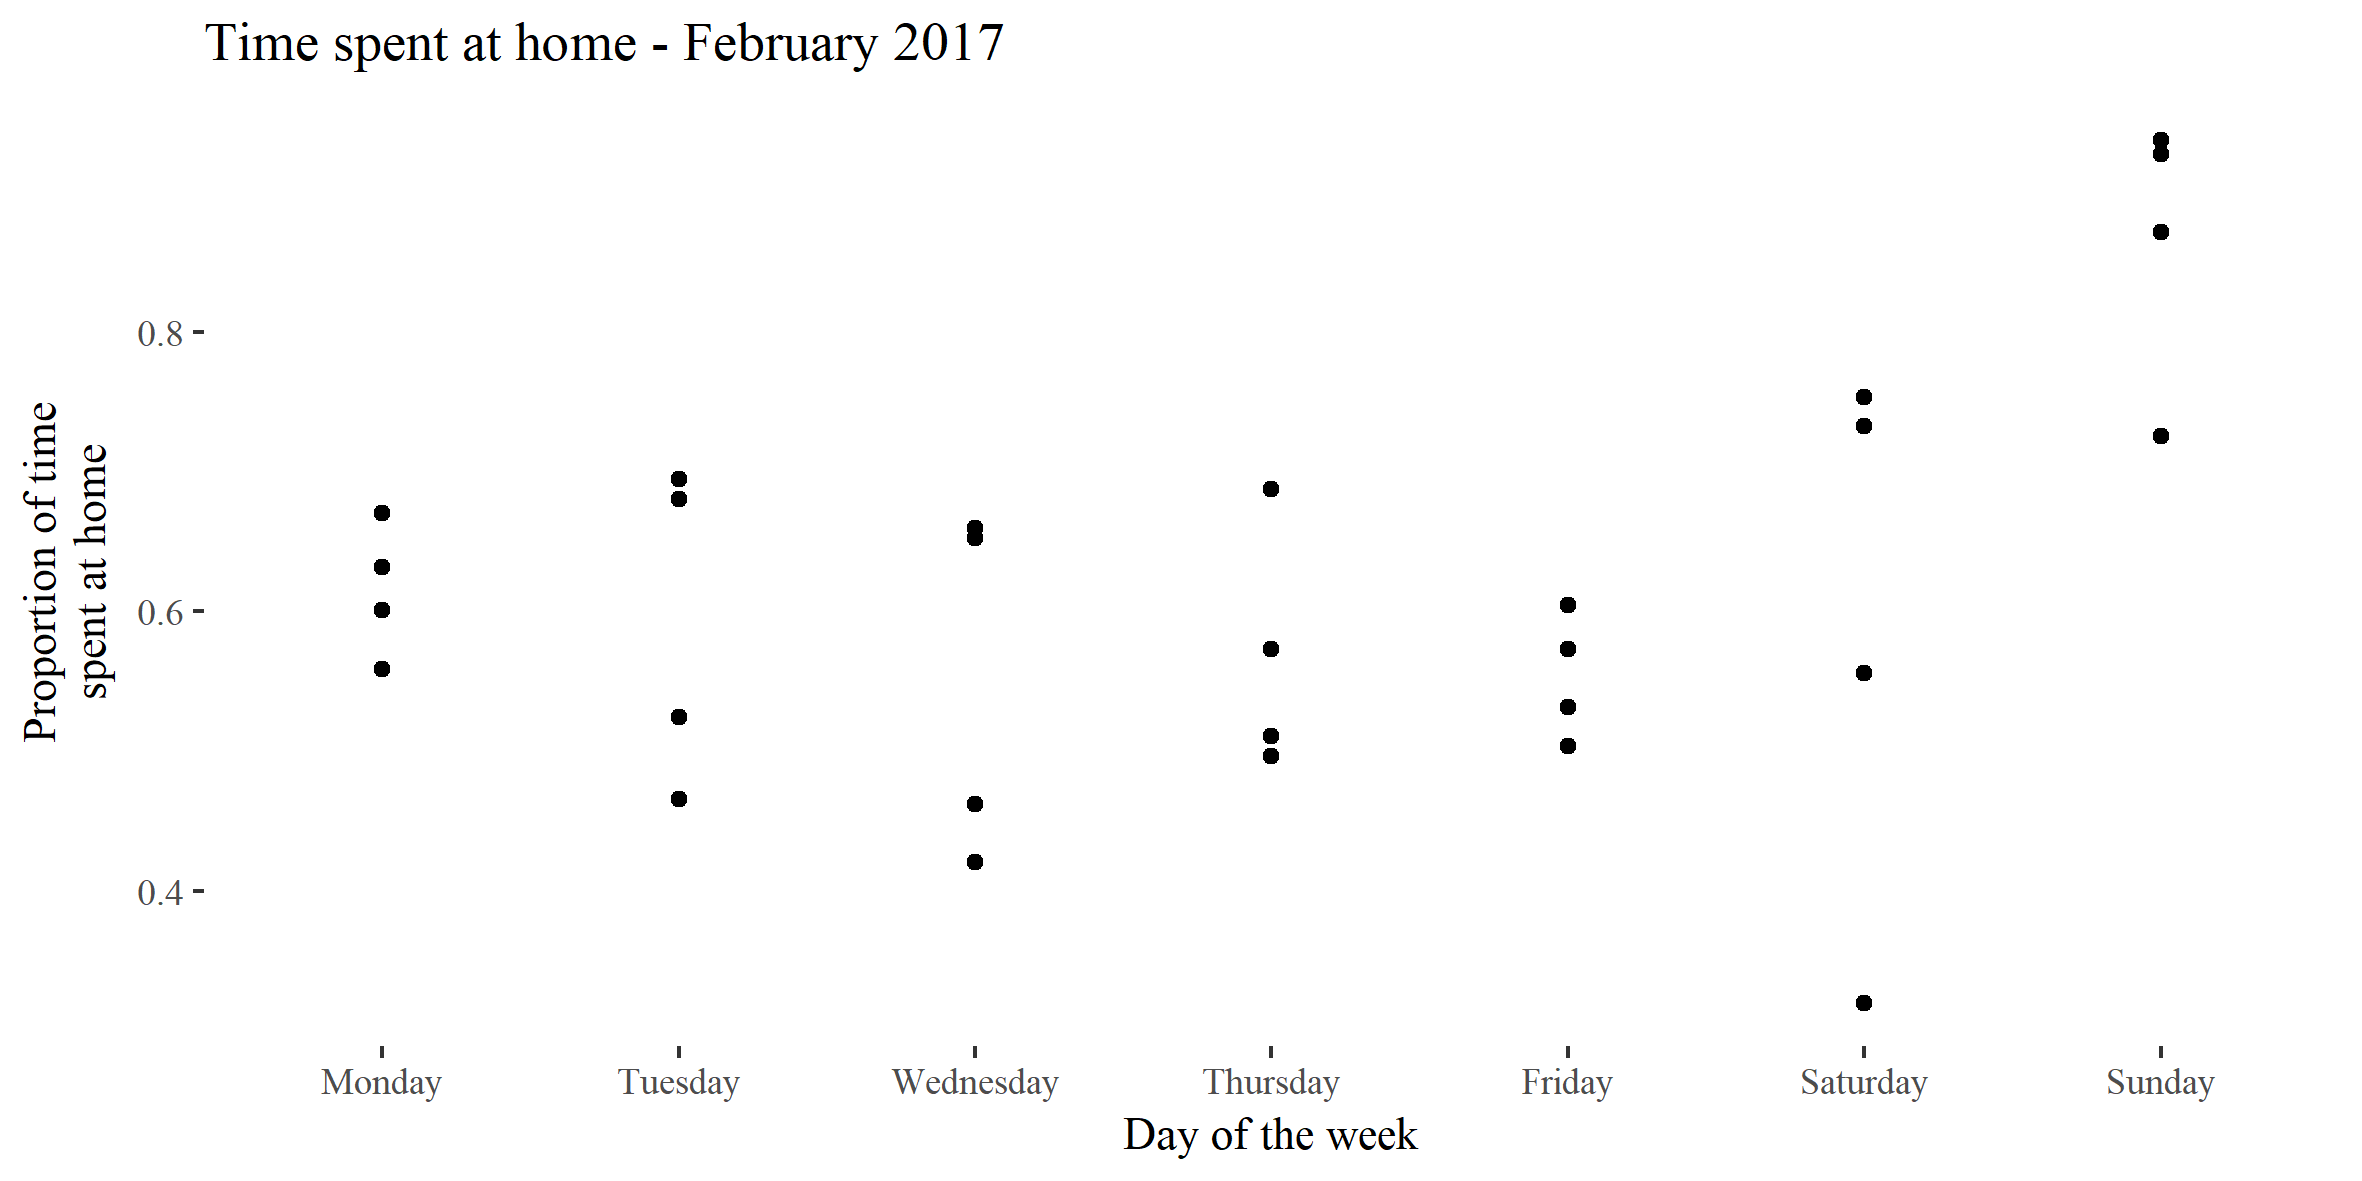
\includegraphics[width=1\linewidth]{img/timeUse} \caption{Proportion of time spent at home in March 2017. The raw values are estimated by downsampling temporally the lattitude and longitude for every 5 minute time period in the month. We used each method's own binning method and classified as at home if the downsampled measurement was within 250 meters from home.}\label{fig:aggrePlot}
\end{figure}

Interestingly, all three models suggest that the user spent
approximately 60\% of their time at home. However, without using any
form of missing data imputation approximately 12\% of the time is
unaccounted for. Given that the amount of time spent at home has been
found to be a reliable predictor of extroversion (G. M. Harari et al.,
2016) and the onset of depressive episodes in bipolar patients (Palmius
et al., 2017) obtaining an accurate value for mobility metrics like this
is highly important to social scientists.

\subsection{Discussion \& Conclusion}\label{discussion-conclusion}

Overall the PMMI performed better than the alternative models,
particularly during longer missing periods and with objective data.
However, it did not perform substantially better than the naive baseline
model. In addition, the comparison to the performance of the
Barnett\&Onella and Palmius models is somewhat unfair, as they were
created for custom logs, not secondary logs. Nonetheless, the comparison
remains valid as they are the closest we found to a missing data
imputation methods in smartphone GPS logs.

In addition to higher accuracy under the conditions typical of secondary
logs, the advantages of PPMI are increased coverage and flexibility for
missing data imputation, robustness to irregular sampling, the ability
to model complex non-linear interactions in its imputations, and the
ability to use historical records to smooth movement noise.

PPMI's increased coverage and flexibility comes from its ability to make
complex non-linear predictions. For instance, in a given missing period
it might make sense to predict that the individual is either at home, or
at the office, or at a shop with equal probability. While PPMI can make
such an imputation, none of the alternative methods can do this.
Moreover, the ability to take the prediction probability values from the
neural network also helps in dealing with uncertainty. A known-drawback
of single imputation is that it takes an imputed value and treats it as
observed. Simple rule-based methods such as Palmius' are essentially
algorithmic single imputation methods. With PPMI it is possible to model
uncertainty using the predicted probabilities of each estimate. For
instance, in the previous example, we could choose to only take
estimates with a high degree of confidence, thus creating confidence
intervals by adding and subtracting the amount of cases where the
location of the individual is ambiguous.

With respect to irregular sampling, alternative methods use temporally
based down-sampling in order to reduce noise. This leads to
deterioration in resolution not only over space, but also over time. A
combination of irregular sampling with the fluctuating accuracy values
can lead to nonsensical results. For instance, consider a case where
there are two inaccurate measurements in movement at 12:00:01 and
12:04:59. Down-sampling over 5 minute periods will lead to a value that
will be the mean of the two inaccurate samples, which is likely to be a
location the individual is certainly not. PPMI instead down-samples
spatially, which ensures that the binned location is one which is
composed of the mean of hundreds of observations, not just the few that
happen within a single period.

While both Barnett and Onnela (2016) and Palmius et al. (2017) use
historical data to smoothen pause locations by clustering pause
locations with with a close degree of spatial proximity, neither of them
do the same for non-pause locations. This may be feasible with high
frequency, regularly sampled short duration logs but creates noise with
secondary logs. Moreover, with secondary logs it is feasible to
spatially \enquote{average out} multiple samples of the same path in
order to recreate it in its entirety. For instance, although the mean
sampling frequency during train travels on the Amsterdam-Utrecht line is
low (about 0.01 Hz) the personalised map manages to recreate the train
line almost perfectly, despite being completely map agnostic.

There are multiple methodological limitations in this paper. Most
importantly, the evaluation methods are imperfect. The golden standard
would be to use at least one highly accurate professional grade GPS
device with high sampling frequency to compare our data to. Until that
is available, the use of public transport data and cross-validation is
just a substitute.

Furthermore, PPMI can be further developed. The map building function,
the assignment function and the classification model remain simplistic
and could be improved.

In map building, the probability of a pause at a given location is
certainly related to other factors, such as the time of the day as well
as the prior history of pauses at that location. These factors are not
taken into account in the pause extraction function. Improved methods
would do well to do so. As for paths, a drawback of the current method
is that the density of the clusters is a function of the clustering
parameter \(d\), the distance between the observed points and their
sampling density. It does not take into account the length of the path
as well as the average sampling frequency of the path. This is an issue
because it can lead to bins to which data points are seldom assigned.
For example, while the Amsterdam-Utrecht line has been mapped out almost
perfectly, many of the clusters along the route have only been assigned
few measurements. This leads to difficulties in the classification part
of the model, as infrequently observed clusters are hard for the model
to predict.

The current assignment function simply assigns each measurement to the
nearest bin. It does not take into account any contextual information
that can be gleaned from the entire movement history of the information,
such as what path they are on. For instance, assume that it is known
that an individual is travelling from point A to point B along path AB,
and there is an inaccurate measurement closest to a cluster which
belongs to path AC. By only taking distance into account, the
measurement can get assigned to the wrong cluster on path AC. An
improvement would be use a Bayesian method, whereby assignment is a
function of both the measurement and a model of the individuals movement
history. In terms of state-space models like the Kalman filter the state
equation would represent a probabilistic representation of where the
individual could be based on the individuals entire movement history.
The space side of the model would be a measurement equation representing
the measurement and the uncertainty surrounding it in the form of \(a\).

As for the simplicity of the classification method, the neural network
which was used to generate predictions used no information on sequence
patterns longer than the previous and next bin. A more sophisticated
recurrent neural network (RNN), or a long short-term memory recurrent
neural network (LSTM) would likely perform significantly better.

That there is room for improvement is unsurprising given that it is
still early days for using smartphone location measurements in social
science. Nonetheless, the methodological advantages are clear: millions
of individuals have a location log containing objective measurements
spanning years which can be accessed for free. This is vastly superior
to alternatives such questionnaires which rely on accurate
self-reporting. Social science researchers must take advantage of
regulatory changes in data portability regulations and put the vast
wealth of data collected by commercial entities to public use.

\newpage

\section{References}\label{references}

\begin{Shaded}
\begin{Highlighting}[]
\KeywordTok{r_refs}\NormalTok{(}\DataTypeTok{file =} \StringTok{"r-references.bib"}\NormalTok{)}
\end{Highlighting}
\end{Shaded}

\begingroup
\setlength{\parindent}{-0.5in} \setlength{\leftskip}{0.5in}

\hypertarget{refs}{}
\hypertarget{ref-R-ggthemes}{}
Arnold, J. B. (2017). \emph{Ggthemes: Extra themes, scales and geoms for
'ggplot2'}. Retrieved from
\url{https://CRAN.R-project.org/package=ggthemes}

\hypertarget{ref-R-papaja}{}
Aust, F., \& Barth, M. (2018). \emph{papaja: Create APA manuscripts with
R Markdown}. Retrieved from \url{https://github.com/crsh/papaja}

\hypertarget{ref-barnett_inferring_2016}{}
Barnett, I., \& Onnela, J.-P. (2016). Inferring mobility measures from
GPS traces with missing data. \emph{arXiv:1606.06328 {[}Stat{]}}.
Retrieved from \url{http://arxiv.org/abs/1606.06328}

\hypertarget{ref-chen_practical_2006}{}
Chen, M. Y., Sohn, T., Chmelev, D., Haehnel, D., Hightower, J., Hughes,
J., \ldots{} Varshavsky, A. (2006). Practical metropolitan-scale
positioning for GSM phones. In \emph{UbiComp 2006: Ubiquitous computing}
(pp. 225--242). Springer, Berlin, Heidelberg.
doi:\href{https://doi.org/10.1007/11853565_14}{10.1007/11853565\_14}

\hypertarget{ref-chen_state_2013}{}
Chen, Z., \& Brown, E. N. (2013). State space model.
\emph{Scholarpedia}, \emph{8}(3), 30868.
doi:\href{https://doi.org/10.4249/scholarpedia.30868}{10.4249/scholarpedia.30868}

\hypertarget{ref-commission_protecting_2017}{}
Commission, E. (2017). \emph{Protecting your data: Your rights -
european commission}. Retrieved from
\url{http://ec.europa.eu/justice/data-protection/individuals/rights/index_en.htm}

\hypertarget{ref-delclos-alio_keeping_2017}{}
Delclòs-Alió, X., Marquet, O., \& Miralles-Guasch, C. (2017). Keeping
track of time: A smartphone-based analysis of travel time perception in
a suburban environment. \emph{Travel Behaviour and Society},
\emph{9}(Supplement C), 1--9.
doi:\href{https://doi.org/10.1016/j.tbs.2017.07.001}{10.1016/j.tbs.2017.07.001}

\hypertarget{ref-duncan_portable_2013}{}
Duncan, S., Stewart, T. I., Oliver, M., Mavoa, S., MacRae, D., Badland,
H. M., \& Duncan, M. J. (2013). Portable global positioning system
receivers: Static validity and environmental conditions. \emph{American
Journal of Preventive Medicine}, \emph{44}(2), e19--29.
doi:\href{https://doi.org/10.1016/j.amepre.2012.10.013}{10.1016/j.amepre.2012.10.013}

\hypertarget{ref-feng_cutoff:_2014}{}
Feng, L., Nowak, G., O'Neill, T., \& Welsh, A. (2014). CUTOFF: A
spatio-temporal imputation method. \emph{Journal of Hydrology},
\emph{519}, 3591--3605.
doi:\href{https://doi.org/10.1016/j.jhydrol.2014.11.012}{10.1016/j.jhydrol.2014.11.012}

\hypertarget{ref-goodchild_toward_2010}{}
Goodchild, M. F., \& Janelle, D. G. (2010). Toward critical spatial
thinking in the social sciences and humanities. \emph{GeoJournal},
\emph{75}(1), 3--13.
doi:\href{https://doi.org/10.1007/s10708-010-9340-3}{10.1007/s10708-010-9340-3}

\hypertarget{ref-grunerbl_smartphone-based_2015}{}
Grünerbl, A., Muaremi, A., Osmani, V., Bahle, G., Ohler, S., Tröster,
G., \ldots{} Lukowicz, P. (2015). Smartphone-based recognition of states
and state changes in bipolar disorder patients. \emph{IEEE Journal of
Biomedical and Health Informatics}, \emph{19}(1), 140--148.
doi:\href{https://doi.org/10.1109/JBHI.2014.2343154}{10.1109/JBHI.2014.2343154}

\hypertarget{ref-harari_using_2016}{}
Harari, G. M., Lane, N. D., Wang, R., Crosier, B. S., Campbell, A. T.,
\& Gosling, S. D. (2016). Using smartphones to collect behavioral data
in psychological science: Opportunities, practical considerations, and
challenges. \emph{Perspectives on Psychological Science}, \emph{11}(6),
838--854.
doi:\href{https://doi.org/10.1177/1745691616650285}{10.1177/1745691616650285}

\hypertarget{ref-jankowska_framework_2015}{}
Jankowska, M. M., Schipperijn, J., \& Kerr, J. (2015). A framework for
using GPS data in physical activity and sedentary behavior studies.
\emph{Exercise and Sport Sciences Reviews}, \emph{43}(1), 48--56.
doi:\href{https://doi.org/10.1249/JES.0000000000000035}{10.1249/JES.0000000000000035}

\hypertarget{ref-lamarca_place_2005}{}
LaMarca, A., Chawathe, Y., Consolvo, S., Hightower, J., Smith, I.,
Scott, J., \ldots{} Schilit, B. (2005). Place lab: Device positioning
using radio beacons in the wild. In \emph{Pervasive computing} (pp.
116--133). Springer, Berlin, Heidelberg.
doi:\href{https://doi.org/10.1007/11428572_8}{10.1007/11428572\_8}

\hypertarget{ref-location_history_timeline_2017}{}
Location History, G. (2017). \emph{Timeline}. Retrieved from
\url{https://www.google.com/maps/timeline?pb}

\hypertarget{ref-london_encoding_2016}{}
London, I. (2016). \emph{Encoding cyclical continuous features - 24-hour
time. Ian london's blog}. Retrieved April 27, 2018, from
\url{//ianlondon.github.io/blog/encoding-cyclical-features-24hour-time/}

\hypertarget{ref-palmius_detecting_2017}{}
Palmius, N., Tsanas, A., Saunders, K. E. A., Bilderbeck, A. C., Geddes,
J. R., Goodwin, G. M., \& Vos, M. D. (2017). Detecting bipolar
depression from geographic location data. \emph{IEEE Transactions on
Biomedical Engineering}, \emph{64}(8), 1761--1771.
doi:\href{https://doi.org/10.1109/TBME.2016.2611862}{10.1109/TBME.2016.2611862}

\hypertarget{ref-patterson_statespace_2008}{}
Patterson, T. A., Thomas, L., Wilcox, C., Ovaskainen, O., \&
Matthiopoulos, J. (2008). State--space models of individual animal
movement. \emph{Trends in Ecology \& Evolution}, \emph{23}(2), 87--94.
doi:\href{https://doi.org/10.1016/j.tree.2007.10.009}{10.1016/j.tree.2007.10.009}

\hypertarget{ref-preisler_modeling_2004}{}
Preisler, H. K., Ager, A. A., Johnson, B. K., \& Kie, J. G. (2004).
Modeling animal movements using stochastic differential equations.
\emph{Environmetrics 15: P. 643-657}. Retrieved from
\url{https://www.fs.usda.gov/treesearch/pubs/33038}

\hypertarget{ref-R-base}{}
R Core Team. (2017). \emph{R: A language and environment for statistical
computing}. Vienna, Austria: R Foundation for Statistical Computing.
Retrieved from \url{https://www.R-project.org/}

\hypertarget{ref-sadilek_far_2016}{}
Sadilek, A., \& Krumm, J. (2016). Far out: Predicting long-term human
mobility. \emph{Microsoft Research}. Retrieved from
\url{https://www.microsoft.com/en-us/research/publication/far-predicting-long-term-human-mobility/}

\hypertarget{ref-saeb_mobile_2015}{}
Saeb, S., Zhang, M., Karr, C. J., Schueller, S. M., Corden, M. E.,
Kording, K. P., \& Mohr, D. C. (2015). Mobile phone sensor correlates of
depressive symptom severity in daily-life behavior: An exploratory
study. \emph{Journal of Medical Internet Research}, \emph{17}(7), e175.
doi:\href{https://doi.org/10.2196/jmir.4273}{10.2196/jmir.4273}

\hypertarget{ref-schipperijn_dynamic_2014}{}
Schipperijn, J., Kerr, J., Duncan, S., Madsen, T., Klinker, C. D., \&
Troelsen, J. (2014). Dynamic accuracy of GPS receivers for use in health
research: A novel method to assess GPS accuracy in real-world settings.
\emph{Frontiers in Public Health}, \emph{2}, 21.
doi:\href{https://doi.org/10.3389/fpubh.2014.00021}{10.3389/fpubh.2014.00021}

\hypertarget{ref-simmons_false-positive_2011}{}
Simmons, J. P., Nelson, L. D., \& Simonsohn, U. (2011). False-positive
psychology: Undisclosed flexibility in data collection and analysis
allows presenting anything as significant. \emph{Psychological Science},
\emph{22}(11), 1359--1366.
doi:\href{https://doi.org/10.1177/0956797611417632}{10.1177/0956797611417632}

\hypertarget{ref-_st-dbscan:_2007}{}
ST-DBSCAN: An algorithm for clustering spatial--temporal data. (2007).
\emph{Data \& Knowledge Engineering}, \emph{60}(1), 208--221.
doi:\href{https://doi.org/10.1016/j.datak.2006.01.013}{10.1016/j.datak.2006.01.013}

\hypertarget{ref-villanueva_association_2013}{}
Villanueva, C., \& Aggarwal, B. (2013). The association between
neighborhood socioeconomic status and clinical outcomes among patients 1
year after hospitalization for cardiovascular disease. \emph{Journal of
Community Health}, \emph{38}(4), 690--697.
doi:\href{https://doi.org/10.1007/s10900-013-9666-0}{10.1007/s10900-013-9666-0}

\hypertarget{ref-wang_smartgpa:_2015}{}
Wang, R., Harari, G., Hao, P., Zhou, X., \& Campbell, A. T. (2015).
SmartGPA: How smartphones can assess and predict academic performance of
college students. In \emph{Proceedings of the 2015 ACM international
joint conference on pervasive and ubiquitous computing} (pp. 295--306).
New York, NY, USA: ACM.
doi:\href{https://doi.org/10.1145/2750858.2804251}{10.1145/2750858.2804251}

\hypertarget{ref-R-ggplot2}{}
Wickham, H. (2009). \emph{Ggplot2: Elegant graphics for data analysis}.
Springer-Verlag New York. Retrieved from \url{http://ggplot2.org}

\hypertarget{ref-wolf_impact_2003}{}
Wolf, J., Oliveira, M., \& Thompson, M. (2003). Impact of underreporting
on mileage and travel time estimates: Results from global positioning
system-enhanced household travel survey. \emph{Transportation Research
Record: Journal of the Transportation Research Board}, \emph{1854},
189--198. doi:\href{https://doi.org/10.3141/1854-21}{10.3141/1854-21}

\hypertarget{ref-R-knitr}{}
Xie, Y. (2015). \emph{Dynamic documents with R and knitr} (2nd ed.).
Boca Raton, Florida: Chapman; Hall/CRC. Retrieved from
\url{https://yihui.name/knitr/}

\hypertarget{ref-zenk_how_2009}{}
Zenk, S. N., Schulz, A. J., \& Odoms-Young, A. (2009). How neighborhood
environments contribute to obesity. \emph{The American Journal of
Nursing}, \emph{109}(7), 61--64.
doi:\href{https://doi.org/10.1097/01.NAJ.0000357175.86507.c8}{10.1097/01.NAJ.0000357175.86507.c8}

\hypertarget{ref-zhang_application_2017}{}
Zhang, Z., Yang, X., Li, H., Li, W., Yan, H., \& Shi, F. (2017).
Application of a novel hybrid method for spatiotemporal data imputation:
A case study of the minqin county groundwater level. \emph{Journal of
Hydrology}, \emph{553}(Supplement C), 384--397.
doi:\href{https://doi.org/10.1016/j.jhydrol.2017.07.053}{10.1016/j.jhydrol.2017.07.053}

\endgroup






\end{document}
